\documentclass{article}

\usepackage{fullpage}
\usepackage{graphicx}
\usepackage{hyperref}
\def\UrlFont{\smaller\ttfamily}
\usepackage{hevea}
\usepackage{fancybox}
\usepackage{relsize}
\usepackage{textcomp}
\usepackage{tabularx}
\usepackage{fancyvrb}
\usepackage{upquote}

% Source code
\newcommand{\expr}[1]{\texttt{#1}}
\newcommand{\setexpr}[1]{\expr{\ttlcb #1\ttrcb}}
\newcommand{\dictexpr}[1]{\expr{\ttlcb #1\ttrcb}}
% It would make this file easier to write and read if I adjusted the
% category code of ' to make it do a different thing within \expr, but
% I couldn't quickly figure out how to do so.
\newcommand{\stringexpr}[1]{\expr{\ttsq #1\ttsq}}
\newcommand{\op}[1]{\expr{#1}}
\newcommand{\kw}[1]{\expr{#1}}

% Left and right curly braces in tt font
% (Using \{ in \tt yields a Roman "{", so don't do that.)
\newcommand{\ttlcb}{\texttt{\char "7B}}
\newcommand{\ttrcb}{\texttt{\char "7D}}
% straight quote
\newcommand{\ttsq}{\texttt{\char 13}}

% Values
\newcommand{\val}[1]{\mytextsf{#1}}
% A string value
\newcommand{\strval}[1]{\textrm{``}\mytextsf{#1}\textrm{''}}
% List value
\newcommand{\liststart}[1]{\structtype{list}{\listelt{#1}}}
\newcommand{\listelt}[1]{\framebox{\strut\val{#1}}}
\newcommand{\emptylist}{\liststart{\strut}}
\newcommand{\listzero}{\liststart{\strut}}
\newcommand{\listone}[1]{\liststart{#1}}
\newcommand{\listtwo}[2]{\liststart{#1}\listelt{#2}}
\newcommand{\listthree}[3]{\liststart{#1}\listelt{#2}\listelt{#3}}
\newcommand{\listfour}[4]{\liststart{#1}\listelt{#2}\listelt{#3}\listelt{#4}}
\newcommand{\listfive}[5]{\liststart{#1}\listelt{#2}\listelt{#3}\listelt{#4}\listelt{#5}}
% Tuple value
\newcommand{\tuplestart}[1]{\structtype{tuple}{\tupleelt{#1}}}
\newcommand{\tupleelt}[1]{\framebox{\strut\val{#1}}}
\newcommand{\emptytuple}{\tuplestart{\strut}}
\newcommand{\tuplezero}{\tuplestart{\strut}}
\newcommand{\tupleone}[1]{\tuplestart{#1}}
\newcommand{\tupletwo}[2]{\tuplestart{#1}\tupleelt{#2}}
\newcommand{\tuplethree}[3]{\tuplestart{#1}\tupleelt{#2}\tupleelt{#3}}
\newcommand{\tuplefour}[4]{\tuplestart{#1}\tupleelt{#2}\tupleelt{#3}\tupleelt{#4}}
% Set value; argument should \emph{not} have commas.
% \newcommand{\setval}[1]{\{{#1}\}}
\newcommand{\setval}[1]{\structtype{set}{\ovalbox{\strut#1}}}
\newcommand{\setzero}{\setval{}}
\newcommand{\setone}[1]{\setval{\val{#1}}}
\newcommand{\settwo}[2]{\setval{\val{#1} ~ \val{#2}}}
\newcommand{\setthree}[3]{\setval{\val{#1} ~ \val{#2} ~ \val{#3}}}
\newcommand{\setfour}[4]{\setval{\val{#1} ~ \val{#2} ~ \val{#3} ~ \val{#4}}}
% Dict value; argument should \emph{not} have commas.
\newcommand{\dictval}[1]{\structtype{dict}{\ovalbox{\strut#1}}}
\newcommand{\dictzero}{\dictval{}}
\newcommand{\dictone}[2]{\dictval{\val{#1}$\rightarrow$\val{#2}}}
\newcommand{\dicttwo}[4]{\dictval{\val{#1}$\rightarrow$\val{#2} ~ \val{#3}$\rightarrow$\val{#4}}}
\newcommand{\dictthree}[6]{\dictval{\val{#1}$\rightarrow$\val{#2} ~ \val{#3}$\rightarrow$\val{#4} ~ \val{#5}$\rightarrow$\val{#6}}}
\newcommand{\dictfour}[8]{\dictval{\val{#1}$\rightarrow$\val{#2} ~ \val{#3}$\rightarrow$\val{#4} ~ \val{#5}$\rightarrow$\val{#6} ~ \val{#7}$\rightarrow$\val{#8}}}

% \newcommand{\structtype}[1]{\makebox[0in][l]{\raisebox{12pt}[0pt]{{\footnotesize \textrm{#1}}}}}
\newlength{\myheight}
\newcommand{\structtype}[2]{%
\settoheight{\myheight}{\hbox{#2}}%
\makebox[0in][l]{\raisebox{\the\myheight}{{\footnotesize \textrm{#1}}}}%
#2}


% Evaluation
\newcommand{\ul}[1]{\underline{#1}}
\newcommand{\RaNospace}{\ensuremath{\Rightarrow}}
\newcommand{\Ra}{ \ensuremath{\Rightarrow} }
\newcommand{\ra}{ \ensuremath{\rightarrow} }
\newcommand{\Da}{ \ensuremath{\Downarrow} }

% Metavariables
\newcommand{\mvar}[1]{\expr{\emph{\uppercase{#1}}}}

% Formatting hacks
\newcommand{\myparagraph}[1]{\paragraph{#1} \ifhevea\else \strut \\ \strut \fi}
\newcommand{\linktotruthvaluetesting}[1]{\ahref{https://docs.python.org/2/library/stdtypes.html\#truth-value-testing}{#1}}
\newcommand{\indentcode}{\indent ~ ~}
\newcommand{\pretabularspace}{\ifhevea\else \strut \\ \strut \fi}
\newcommand{\posttabularspace}{\ifhevea\else \strut \\ \strut \fi}

% Sans serif font in Hevea.
\ifhevea
% \newcommand{\mytextsf}[1]{%
%   \begin{rawhtml}<span style="font-family:sans-serif">\end{rawhtml}%
%   #1%
%   \begin{rawhtml}</span>\end{rawhtml}}
\newcommand{\mytextsf}[1]{{\@span{style="font-family:sans-serif"}#1}}
\else
\newcommand{\mytextsf}[1]{\textsf{#1}}
\fi


\setcounter{tocdepth}{2}

\begin{document}

\title{Python Evaluation Rules}
\author{Michael Ernst and Isaac Reynolds \\
 mernst@cs.washington.edu
}

\maketitle

\tableofcontents

\centerline{}

\section{Introduction}


This document presents step-by-step rules for executing a Python program. A
skilled Python programmer uses these rules to reason about the effects of
Python code. This document will enable you to program more efficiently and
with less confusion.

We wrote this document as a reaction to
the vague English descriptions in many textbooks and websites.
If you have only a fuzzy notion of what Python does, you will struggle to write
correct code, debug incorrect code, and read unfamiliar code.
This document might take some effort to understand on first reading, but
overall it will save you time and avoid frustration.

This document applies to both Python 2 and Python 3.
It does not cover every possible Python expression, but does cover the
most frequently-used ones.

This document was originally written in fall 2011 for use in 
\href{http://tinyurl.com/dataprogramming}{UW CSE 160}.


\subsection{The Structure of a Python Program}

  A Python \textbf{program} is a sequence of statements. Python executes this sequence of statements in a specific, consistent, and predictable order.

  A Python \textbf{statement} contains zero or more expressions. A statement typically has a side effect such as printing output, computing a useful value, or changing which statement is executed next.

A Python \textbf{expression} describes a computation, or operation,
performed on data.  For example, the arithmetic expression \expr{2+1}
describes the operation of adding \val{1} to \val{2}.  An expression may
contain sub-expressions --- the expression \expr{2+1} contains the
sub-expressions \expr{2} and \expr{1}.

An expression is some text a programmer writes, and a \textbf{value} is
Python's internal representation of a piece of data. Evaluating an
expression computes a Python \textbf{value}. This means that the Python
expression \expr{2} is different from the value \val{2}.  This document
uses \expr{typewriter font} for statements and expressions and \val{sans
  serif font} for values.

\subsection{How to Execute a Python Program}

Python executes a \textbf{program} by executing the program's statements
one by one until there are no more statements left to execute. In general,
Python executes statements from top to bottom.

  Python executes a \textbf{statement} by evaluating its expressions to values one by one, then performing some operation on those values.

Python evaluates an \textbf{expression} by first evaluating its
sub-expressions, then performing an operation on the values. Notice that
each sub-expression might have its own sub-sub-expressions, so this
process might repeat several times. However, this process of dividing and
evaluating always terminates because the expressions become smaller at
each step until they reach some base expression.

For example, to evaluate \expr{2*10 + 6/3}, Python first evaluates
\expr{2*10} to the value \val{20}, then evaluates \expr{6/3} to the value
\val{2}, then adds the two to get \val{22}.  Note that in order to evaluate
one expression, Python evaluates several smaller expressions (such as
\expr{2*10}). Furthermore, to evaluate \expr{2*10},  Python evaluates the
expression \expr{2} to the value \val{2}, and so forth.  The value of a
literal expression such as \expr{2} is the corresponding value, so this is
where Python stops dividing into sub-expressions.

The remainder of this document gives evaluation rules for Python expressions and
statements.

The general approach is \emph{rewriting}.  Given a statement or expression,
each individual rule does a tiny bit of work that simplifies the statement
or expression to an equivalent but shorter or simpler version, until there
is no more work to do and you have executed the whole thing.  The general
idea is to break up an imposing task into bite-sized pieces.  Evaluation of
any program proceeds by small, simple steps, and by understanding these you
can understand the execution of the whole program.


\bigskip

Comments and corrections to this document are welcome; send them to
mernst@cs.washington.edu.


\section{Literal Expressions}

  A literal expression evaluates to the value it represents. Here are some examples of literal expressions and the values to which they evaluate:

  \pretabularspace
  \begin{tabular}{l c l}
  \expr{17} & \Ra & \val{17} \\
  \stringexpr{this is some text} & \Ra & \strval{this is some text} \\
  \expr{8.125} & \Ra & \val{8.125} \\
  \expr{True} & \Ra & \val{True} \\
  \end{tabular}
  \posttabularspace

  This document uses {\RaNospace} to show an expression (on the left) and the value to
  which it evaluates (on the right).

\section{Operator Expressions}
\subsection{Binary Expressions}

A binary expression consists of a binary operator applied to two operand
expressions. A binary operator is an operator that takes two arguments (for
example, \op{+} or \op{/}). Here are some examples of binary arithmetic
expressions, each of which evaluates to a number:

  \pretabularspace
  \begin{tabular}{l c l}
  \expr{2 * 5} & \Ra & \val{10} \\
  \expr{14 + 8} & \Ra & \val{22} \\
  \end{tabular}
  \posttabularspace

Here are some examples of binary Boolean expressions, each of which
evaluates to a Boolean (\val{True} or \val{False}):

  \pretabularspace
  \begin{tabular}{l c l}
  \expr{6 == 7} & \Ra & \val{False} \\
  \expr{0 < 5} & \Ra & \val{True} \\
  \expr{True and False} & \Ra & \val{False} \\
  \end{tabular}
  \posttabularspace

  Some expressions don't evaluate to numbers or Booleans. For instance, applying the \op{+} operator to two string values evaluates to the concatenation of the two strings:

  \pretabularspace
  \begin{tabular}{l c l}
  \expr{\stringexpr{have a } + \stringexpr{very good day}} & \Ra & \strval{have a very good day} \\
  \end{tabular}
  \posttabularspace

  In general, a binary expression has the form:

  \pretabularspace
  \mvar{EXPR BIN\_OP EXPR}

\subsubsection{Rules for Evaluation}

  To evaluate a binary expression to a value,

  \begin{enumerate}
    \item
    Evaluate the left operand (which is an expression) to a value and replace that operand expression with that value.

    \item
    Evaluate the right operand (which is an expression) to a value and replace that operand expression with that value.

    \item
    Apply \mvar{BIN\_OP} to the two resultant values, obtaining the value of the binary expression. Replace the entire binary expression with this value.

  \end{enumerate}

\subsubsection{Examples}

  Below are some examples of evaluating binary expressions. Each example starts with a binary expression and shows each step of the evaluation, ending with the value to which the binary expression evaluates. The underlined part of each expression is the part that is evaluated next.

  Remember that expressions are in \expr{typewriter font} and values are in \val{sans serif font}.

  \begin{enumerate}
    \item \expr{\ul{2} * 5} \\
      \expr{\val{2} * \ul{5}} \\
      \expr{\ul{\val{2} * \val{5}}} \\
      \val{10}

    \item \expr{\ul{14} + 8} \\
      \expr{\val{14} + \ul{8}} \\
      \expr{\ul{\val{14} + \val{8}}} \\
      \val{22}

    \item \expr{\ul{True} and False} \\
      \expr{\val{True} and \ul{False}} \\
      \expr{\ul{\val{True} and \val{False}}} \\
      \val{False}

    \item \expr{\ul{\stringexpr{have a }} + \stringexpr{very good day}} \\
      \expr{\strval{have a } + \ul{\stringexpr{very good day}}} \\
      \expr{\ul{\strval{have a } + \strval{very good day}}} \\
      \strval{have a very good day}
  \end{enumerate}

\subsection{Compound Expressions}
\label{compoundexpressions}

When at least one of the operands is itself an expression (as in \expr{2 *
  5 + 1}), the expression is a compound expression. Python follows the
standard mathematical order of operations, so \expr{2 * 5 + 1} is
equivalent to \expr{(2 * 5) + 1}. Here are some examples of compound
expressions:

  \pretabularspace
  \begin{tabular}{l c l}
  \expr{2 * 5 + 1} & \Ra & \val{11} \\
  \expr{2 + 5 - 1} & \Ra & \val{6} \\
  \expr{4 * 6 / 8} & \Ra & \val{3} \\
  \expr{True and not False} & \Ra & \val{True} \\
  \end{tabular}

  You can use parentheses to override Python's order of operations, or just for
  clarity. A parenthetical expression has the form:

  \pretabularspace
  \mvar{(EXPR)}
  \posttabularspace

A parenthetical expression evaluates to the same value as the enclosed
subexpression, \mvar{EXPR}, does. For example, \expr{(22)} evaluates to
the same thing \expr{22} does, namely \val{22}.  As another example,

  \pretabularspace
  \begin{tabular}{l c r}
  \expr{2 * (5 + 1)} & \Ra & \val{12}
  \end{tabular}

\subsubsection{Rules for Evaluation}

  To evaluate a compound expression to a value,

  \begin{enumerate}
    \item
    Use order of operations to identify the main operator (the last operator that you'll apply). For example, the main operator in \expr{2 * 5 + 1} is \op{+}, so \expr{2 * 5 + 1} is an addition expression.

    \item
    Identify the operands to the main operator. Then evaluate this expression (the main operator and its two operands) as you would evaluate a binary expression.

  \end{enumerate}

\subsubsection{Examples}

  Below are examples of evaluating compound expressions.

  \begin{enumerate}
    \item
      \expr{\ul{\ul{3} * 6} + 7} \\
      \expr{\ul{\val{3} * \ul{6}} + 7} \\
      \expr{\ul{\val{3} * \val{6}} + 7} \\
      \expr{\val{18} + \ul{7}} \\
      \expr{\ul{\val{18} + \val{7}}} \\
      \val{25}

      This example contains some extra underlining to emphasize the
      following.  To evaluate \expr{3 * 6 + 7}, it is necessary to first
      evaluate its left-hand side, \expr{3 * 6}.  To evaluate \expr{3 * 6},
      it is necessary to first evaluate \emph{its} left-hand side,
      \expr{3}.

    \item
      \expr{\ul{6} + 7 + 8} \\
      \expr{\val{6} + \ul{7} + 8} \\
      \expr{\ul{\val{6} + \val{7}} + 8} \\
      \expr{\val{13} + \ul{8}} \\
      \expr{\val{13} + \val{8}} \\
      \val{21}

      To simplify this document, from now on we will sometimes elide some
      steps if they are obvious.  For instance, the following example goes
      straight from \expr{6 < 0} to \val{False}.

    \item \expr{\ul{6 < 0} or 6 > 10} \\
      \expr{\val{False} or \ul{6 > 10}} \\
      \expr{\ul{\val{False} or \val{False}}} \\
      \val{False}

%     \item \expr{\ul{2} * -3} \\
%       \expr{\val{2} * \ul{-3}} \\
%       \expr{\ul{\val{2} * \val{-3}}} \\
%       \val{-6}
  \end{enumerate}

\subsection{Unary Expressions}

  A unary operator operates on a single value. In general, a unary expression has the form:

  \pretabularspace
  \mvar{UN\_OP EXPR}
  \posttabularspace

  Two common unary operators are \kw{not} and \op{-}. The \kw{not} operator negates a Boolean value; for example, \expr{not False} evaluates to \val{True}. Used as a unary operator, the \op{-} operator negates a numerical value; for example, \expr{-(2 * 5)} evaluates to \val{-10}.

\subsubsection{Rules for Evaluation}

  To evaluate a unary expression to a value,

  \begin{enumerate}
    \item
    Evaluate \mvar{EXPR} to a value and replace \mvar{EXPR} with that value.

    \item
    Apply \mvar{UN\_OP} to the value and replace the entire expression with the new value.
  \end{enumerate}

\subsubsection{Examples}

  Below are examples of evaluating unary expressions.

  \begin{enumerate}
    \item \expr{-(\ul{12 + 4})} \\
    \expr{-\ul{(\val{16})}} \\
    \expr{\ul{-\val{16}}} \\
    \val{-16}

    \item \expr{-(\ul{1-2})} \\
    \expr{-\ul{(\val{-1})}} \\
    \expr{\ul{- \val{-1}}} \\
    \val{1}

    \item \expr{1 + -\ul{3}} \\
    \expr{1 + \ul{-\val{3}}} \\
    \expr{\ul{1 + \val{-3}}} \\
    \val{-2}

    \item \expr{not \ul{True}} \\
    \ul{\expr{not} \val{True}} \\
    \val{False}
  \end{enumerate}

\section{Variables}

Think of a variable as a container.  A variable stores a value so that you
can reuse it later in your program.  This reduces redundancy, improves
performance, and makes your code more readable.  In order to use a
variable, you first store a value in the variable by \emph{assigning} the
variable to this value.  Later, you \emph{access} that variable, which
looks up the value you assigned to it.  It is an error to access a variable
that has not yet been assigned.  You can reassign a variable --- that is,
give it a new value --- any number of times.

Note that Python's concept of a variable is different from the mathematical
concept of a variable.  In math, a variable's value is fixed and determined
by a mathematical relation.  In Python, a variable is assigned a specific
value at a specific point in time, and it can be reassigned to a different
value later during a program's execution.

Python stores variables and their values in a structure called a
\emph{frame}.  A frame contains a set of \emph{bindings}.  A binding is a
relationship between a variable and its value.  When a program assigns a
variable, Python adds a binding for that variable to the frame (or updates
its value if the variable already exists).  When a program accesses a
variable, Python uses the frame to find a binding for that variable.

Below is an illustration of a Python frame with bindings for 5 variables:

  \pretabularspace
  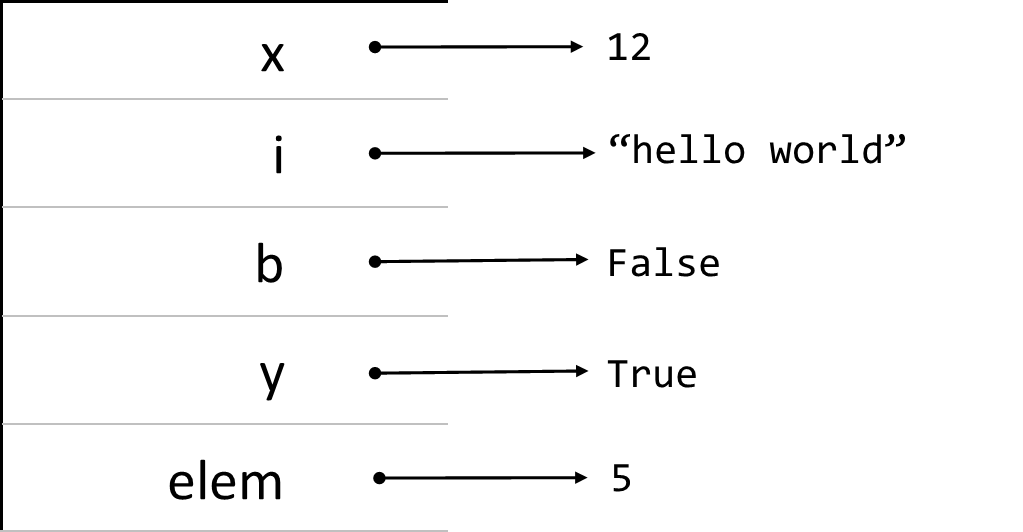
\includegraphics{diagrams/bindings-2}
  \posttabularspace

  For now, this document will consider simple variable assignments and accesses. For a program with functions and function calls, Section~\ref{functions} defines more complete procedures for variable assignments and accesses.

\subsection{Variable Access Expressions}
\label{variableaccessexpressions}

Variable access expressions let you use the value of a variable you've
assigned.  Suppose that the frame is the one illustrated above, where a
variable with the name \expr{x} is assigned the value \val{13}.  Then the
expression \expr{x} evaluates to the value \val{13}.  Here are some
examples of variable access expressions:

  \pretabularspace
  \begin{tabular}{l c l}
  \expr{answer} & \Ra & \val{42} \\
  \expr{(answer + 2) / 2} & \Ra & \val{22} \\
  \end{tabular}
  \posttabularspace

  In general, a variable access expression has the form:

  \pretabularspace
  \mvar{VAR\_EXPR}

For now, \mvar{VAR\_EXPR} is a variable name.
Section~\ref{datastructure-access} generalizes this assumption, enabling
accessing of data structures, as in the expression \expr{mylist[22]}.


\subsubsection{Rules for Evaluation}
\label{variableaccessexpressions-rules}



  To evaluate a variable access expression to a value, search the frame for a binding from \mvar{var\_expr} to a value. If such a binding exists, replace the access expression with that variable's value. Otherwise raise an error, because the variable is not defined.

  Later, Section~\ref{functions} introduces Python functions. When accessing variables in the body of a function, use the refined rules for evaluation in Section~\ref{accesseswithfunctions}.

\subsubsection{Examples}

  Below are examples of evaluating variable access expressions. Each example's first line is the variable access expression, and the second is the value to which that expression evaluates. The examples are evaluated in the context of the frame presented above:

  \begin{enumerate}
    \item \expr{x} \\
    \val{12}

    \item \expr{i} \\
    \strval{hello world}

    \item \expr{o} \\
    ERROR. The variable \expr{o} is not defined.

    \item \expr{y} \\
    \val{True}
  \end{enumerate}

\subsection{Variable Assignment Statements}

  An assignment statement creates a variable and sets its value, or changes the value of an existing variable. Here are some examples of assignments:

\begin{verbatim}
  x = 18
  y = x + 1
  y = y * 2
\end{verbatim}

  In general, an assignment statement has the form:

  \pretabularspace
  \expr{\mvar{VAR\_EXPR} = \mvar{EXPR}}
  \posttabularspace

\subsubsection{Rules for Evaluation}

  To execute an assignment statement,

  \begin{enumerate}
    \item
    Evaluate \mvar{EXPR} to a value and replace \mvar{EXPR} with that value.

    \item
    If the variable already exists in the frame,
    change its binding so that it now refers to the value from the previous step.
    Otherwise, create a new variable in the current frame and bind it to the value from
    the previous step.
  \end{enumerate}

Note that an assignment statement is treated differently from expressions.
For most expressions (such as \expr{x + 18}), both of the subexpressions
are evaluated to a value, then a math operation is performed.  For an
assignment, the right-hand side is evaluated to a value, but the left-hand
side is treated as a name rather than evaluated.

The left-hand side can be more complex than simply a name.
Section~\ref{datastructures} will show how to evaluate an assignment such
as \expr{mylist[22] = \mvar{EXPR}}.

  When assigning variables in the body of a function, use the refined rules for evaluation in Section~\ref{assignmentswithfunctions}.

\subsubsection{Examples}

Below are examples of executing variable assignment statements.
Each example is executed in the context of this frame, unaffected by previous examples:

  \pretabularspace
  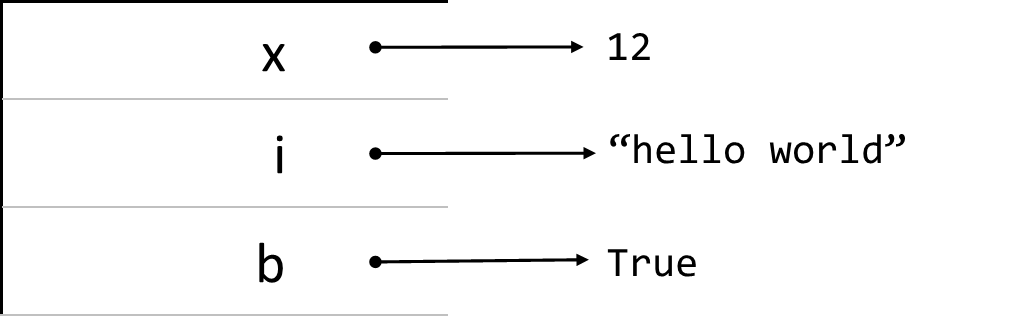
\includegraphics{diagrams/bindings-1.png}
  \posttabularspace

Each example shows the final frame.

  \begin{enumerate}
    \item \expr{var = 18} \\
    Binds new variable \expr{var} to \val{18}.
    \pretabularspace
    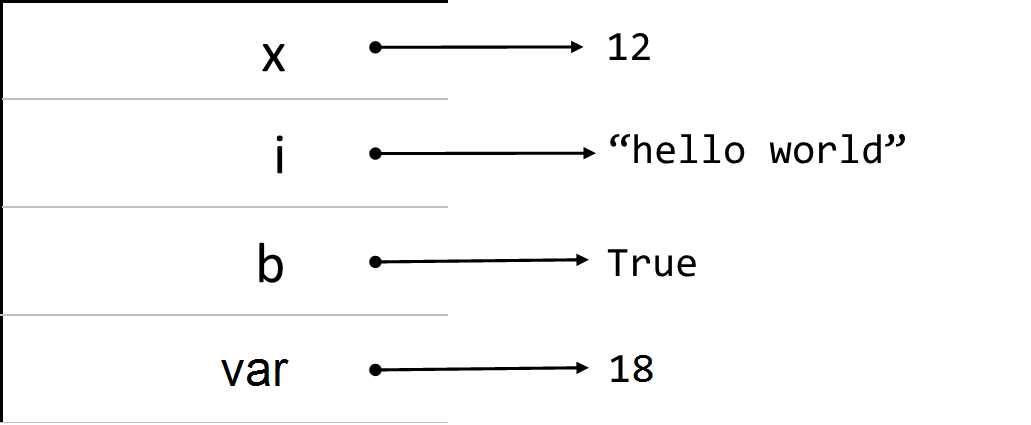
\includegraphics[scale=0.35]{diagrams/bindings-1-1}
    \posttabularspace

    \item \expr{x = 18} \\
    Re-binds \expr{x} to \val{18}.
    \pretabularspace
    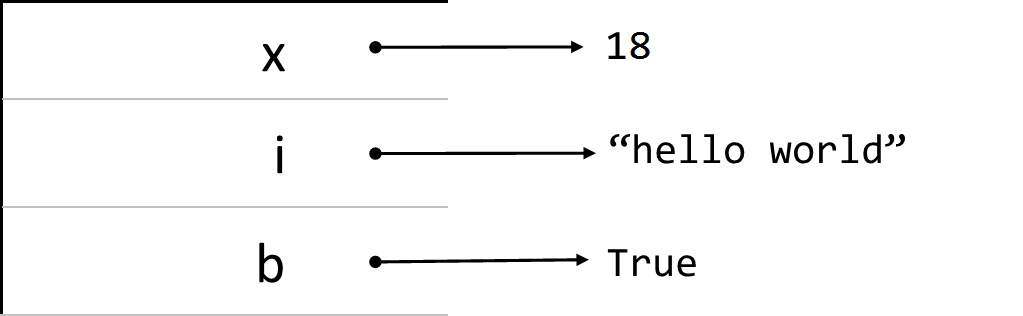
\includegraphics[scale=0.35]{diagrams/bindings-1-2}
    \posttabularspace

    \item \expr{x = i} \\
    Evaluates \expr{i} to \strval{hello world}, then re-binds \expr{x} to that value.
    \pretabularspace
    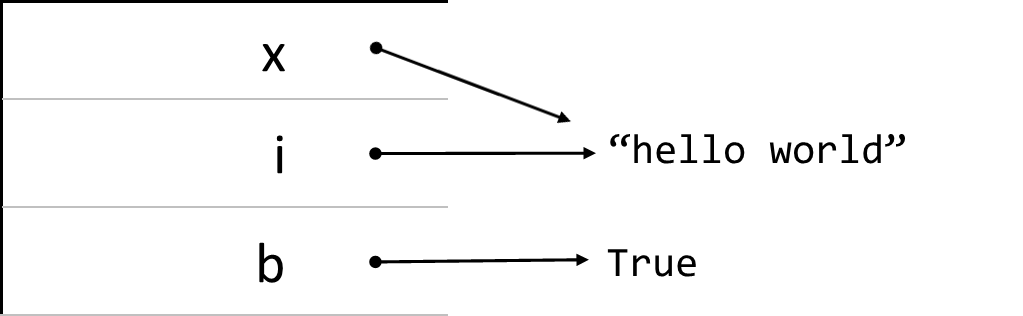
\includegraphics[scale=0.35]{diagrams/bindings-1-3}
    \posttabularspace

    \item \expr{x = x + 1} \\
    Evaluates \expr{x + 1} to \val{13}, then re-binds \expr{x} to that value.
    \pretabularspace
    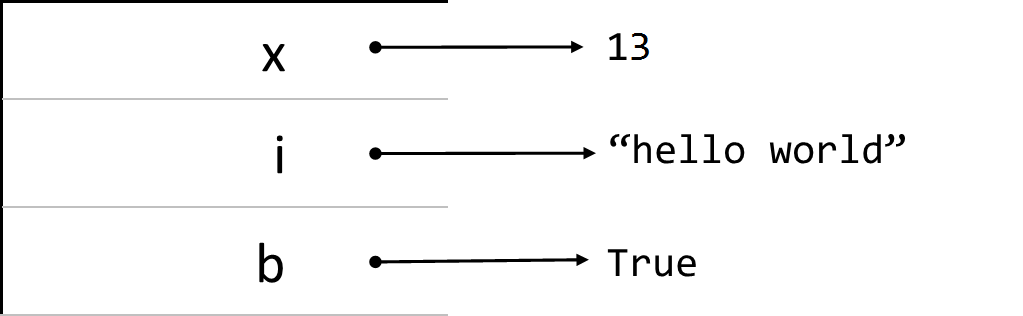
\includegraphics[scale=0.35]{diagrams/bindings-1-4}
    \posttabularspace

  \end{enumerate}

\section{\kw{If} Statements}

An \kw{if} statement lets you execute code only in certain cases (for
example, only if a particular variable is less than \val{0}).  For example,
here's an \kw{if} statement that computes the absolute value of a variable
\expr{x}.

\begin{verbatim}
# x is some number
if x >= 0:
    y =  x
else:
    y = -x
# y is |x|
\end{verbatim}

  An \kw{if} statement consists of a series of \kw{if}, \kw{elif}, and \kw{else} clauses. Every clause (except \kw{else}) consists of a condition (a Boolean expression) and a body (a sequence of statements). In general, an \kw{if} statement has the form:

  \pretabularspace
  \noindent \expr{if \mvar{BOOL\_EXPR}:} \\
  \indent \mvar{BODY\_STATEMENTS} \\
  \noindent \expr{elif \mvar{BOOL\_EXPR}:} \\
  \indent \mvar{BODY\_STATEMENTS} \\
  \noindent \expr{elif \mvar{BOOL\_EXPR}:} \\
  \indent \mvar{BODY\_STATEMENTS} \\
  \noindent \vdots \\
  \noindent \expr{else:} \\
  \indent \mvar{BODY\_STATEMENTS}
  \posttabularspace

  An \kw{if} statement always has exactly one leading \kw{if} clause, zero or more \kw{elif} clauses that follow it, and zero or one \kw{else} clause at the end.

\subsection{Rules for Evaluation}

  In general, Python evaluates the clauses' conditions in order until one evaluates to \val{True}, and then executes only the statements in that clause (and not in any later clause, even if a later clause's condition is also true). To execute an \kw{if} statement,

  \begin{enumerate}
    \item
    If an \kw{else} clause exists, replace it with an \kw{elif True} clause.

    \item
    For each clause, from top to bottom, do the following:
    \begin{enumerate}
      \item Evaluate the current clause's condition to a Boolean value
        (that is, \val{True} or \val{False}) and replace the condition with
        that value.
        If the condition evaluates to a non-Boolean value,
        \linktotruthvaluetesting{convert the value to a Boolean value} (see
        \url{https://docs.python.org/2/library/stdtypes.html\#truth-value-testing}).

      \item
      Choose one of the following:
      \begin{description}
        \item[If the condition evaluates to \val{True}] Execute the statements inside this clause, then end execution of the \kw{if} statement. Ignore all subsequent clauses.

        \item[If the condition evaluates to \val{False}] Ignore this clause and continue to the next clause. If there is no remaining clause, end execution of the \kw{if statement}.
      \end{description}
    \end{enumerate}
  \end{enumerate}

\subsection{Examples}

  Below are examples of executing \kw{if} statements. Each example shows an \kw{if} statement and a timeline that shows how Python evaluates that \kw{if} statement, and ends by showing the body statements that Python will execute.  The examples are evaluated in the context of the following frame.

Each example is executed in the context of this frame, unaffected by previous examples:

  \pretabularspace
  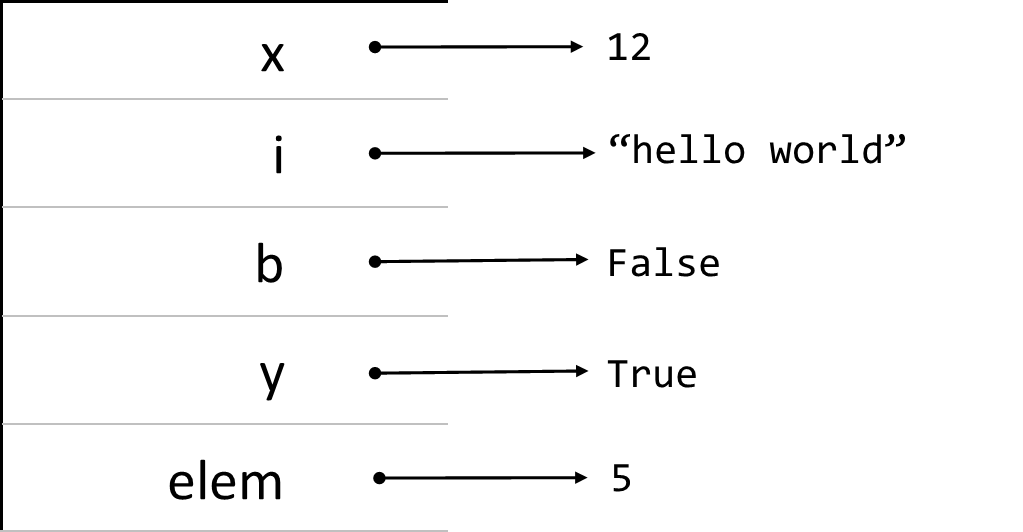
\includegraphics{diagrams/bindings-2.png}
  \posttabularspace

  \begin{enumerate}
    \item
      \expr{if \ul{y}:} \\
      \indentcode \mvar{BODY\_STATEMENTS} \\
      \Da \\
      \expr{if} \val{True}\expr{:} \\
      \indentcode \ul{\mvar{BODY\_STATEMENTS}} \\
      \strut \\
      The first clause is executed, because \expr{y} evaluates to \val{True}.

    \item
      \expr{if \ul{b}:} \\
      \indentcode \mvar{BODY\_STATEMENTS} \\
      \Da \\
      (Nothing) \\
      \strut \\
      No clause is executed, because \expr{b} evaluates to \val{False}.

    \item
      \expr{if not b:} \\
      \indentcode \mvar{BODY\_STATEMENTS} \\
      \expr{\ul{else:}} \\
      \indentcode \mvar{BODY\_STATEMENTS} \\
      \Da \\
      \expr{if \ul{not b}:} \\
      \indentcode \mvar{BODY\_STATEMENTS} \\
      \expr{elif True:} \\
      \indentcode \mvar{BODY\_STATEMENTS} \\
      \Da \\
      \expr{if} \val{True}\expr{:} \\
      \indentcode \mvar{\ul{BODY\_STATEMENTS}} \\
      \expr{elif True:} \\
      \indentcode \mvar{BODY\_STATEMENTS} \\
      \strut \\
      The first clause is executed because \expr{not b} evaluates to \val{True}

    \item
      \expr{if b:} \\
      \indentcode \mvar{BODY\_STATEMENTS} \\
      \expr{\ul{else}:} \\
      \indentcode \mvar{BODY\_STATEMENTS} \\
      \Da \\
      \expr{if \ul{b}:} \\
      \indentcode \mvar{BODY\_STATEMENTS} \\
      \expr{elif True:} \\
      \indentcode \mvar{BODY\_STATEMENTS} \\
      \Da \\
      \expr{if} \val{False}\expr{:} \\
      \indentcode \mvar{BODY\_STATEMENTS} \\
      \expr{elif \ul{True}:} \\
      \indentcode \mvar{BODY\_STATEMENTS} \\
      \Da \\
      \expr{if} \val{False}\expr{:} \\
      \indentcode \mvar{BODY\_STATEMENTS} \\
      \expr{elif} \val{True}\expr{:} \\
      \indentcode \mvar{\ul{BODY\_STATEMENTS}} \\
      \strut \\
      The second clause is executed because \expr{b} evaluates to \val{False}.

   \item
      \expr{if \ul{x < 0}:} \\
      \indentcode \mvar{BODY\_STATEMENTS} \\
      \expr{elif x == 0:} \\
      \indentcode \mvar{BODY\_STATEMENTS} \\
      \expr{elif x > 0:} \\
      \indentcode \mvar{BODY\_STATEMENTS} \\
      \Da \\
      \expr{if} \val{False}\expr{:} \\
      \indentcode \mvar{BODY\_STATEMENTS} \\
      \expr{elif \ul{x == 0}:} \\
      \indentcode \mvar{BODY\_STATEMENTS} \\
      \expr{elif x > 0:} \\
      \indentcode \mvar{BODY\_STATEMENTS} \\
      \Da \\
      \expr{if} \val{False}\expr{:} \\
      \indentcode \mvar{BODY\_STATEMENTS} \\
      \expr{elif} \val{False}\expr{:} \\
      \indentcode \mvar{BODY\_STATEMENTS} \\
      \expr{elif \ul{x > 0}:} \\
      \indentcode \mvar{BODY\_STATEMENTS} \\
      \Da \\
      \expr{if} \val{False}\expr{:} \\
      \indentcode \mvar{BODY\_STATEMENTS} \\
      \expr{elif} \val{False}\expr{:} \\
      \indentcode \mvar{BODY\_STATEMENTS} \\
      \expr{elif} \val{True}\expr{:} \\
      \indentcode \mvar{\ul{BODY\_STATEMENTS}} \\
      \strut \\
      The third clause is executed because \expr{x < 0} evaluates to \val{False}, \expr{x == 0} evaluates to \val{False}, and \expr{x > 0} is \val{True}.

    \item
      \expr{if x > 0:} \\
      \indentcode \mvar{BODY\_STATEMENTS} \\
      \expr{if x == 12:} \\
      \indentcode \mvar{BODY\_STATEMENTS} \\
      \expr{\ul{else}:} \\
      \indentcode \mvar{BODY\_STATEMENTS} \\
      \Da \\
      \expr{if \ul{x > 0}:} \\
      \indentcode \mvar{BODY\_STATEMENTS} \\
      \expr{if x == 12:} \\
      \indentcode \mvar{BODY\_STATEMENTS} \\
      \expr{elif True:} \\
      \indentcode \mvar{BODY\_STATEMENTS} \\
      \Da \\
      \expr{if} \val{True}\expr{:} \\
      \indentcode \mvar{\ul{BODY\_STATEMENTS}} \\
      \expr{if x == 12:} \\
      \indentcode \mvar{BODY\_STATEMENTS} \\
      \expr{elif True:} \\
      \indentcode \mvar{BODY\_STATEMENTS} \\
      \strut \\
      The first clause is executed because \expr{x > 0} evaluates to \val{True}.
  \end{enumerate}

\section{Data structures:  Lists, Tuples, Sets, and Dictionaries}
\label{datastructures}

So far, each value we have seen is a single datum, such as an integer,
decimal number, or Boolean. Python also supports compound values, or data
structures.  A data structure contains multiple values.  Examples include
strings, lists, tuples, sets, and dictionaries.

  \myparagraph{Types of data structures} \strut

  A \textbf{string} is a list of characters. It is used to represent text. Strings also have a corresponding literal constructor (such as \expr{"a string"}).

  A \textbf{tuple} contains any number of elements (but usually only two or three). Some functions return tuples when it is convenient to return a pair of values instead of just one. Tuples are immutable, which means they cannot be changed after they're created. The values in a tuple need not be of the same type, but the values are related --- for instance, a tuple might contain a string that represents a word and the number of times that word appears in a particular text file.

  Here is an example of a 2-tuple whose elements are a word and the number of times that word appears in a text file: \tupletwo{the}{1112}.

A \textbf{list} is an ordered sequence of elements. A list generally
contains many elements of the same type.  Lists are used when order is
important (for instance, sorting) or when it is necessary to keep multiple
instances of a particular element.  Once you have created a list, you can
change, add, and remove elements.

  Here is an example of a list of words in alphabetical order: \listfour{\strval{fun}}{\strval{is}}{\strval{programming}}{\strval{Python}}.

  Strings, tuples, and lists are all \textbf{sequences}. A sequence stores elements in a fixed order by giving each element a unique integer index in the interval [0, $n$-1], where $n$ is the length of the sequence. The first element has index 0, and the last has index $n$-1. You can access a particular element in a sequence by using that element's index; for example, the expression \expr{mylist[0]} evaluates to the first element in the list \expr{mylist}.

A \textbf{set} is an unordered collection of unique elements.  Python
ensures uniqueness for you --- adding to the set an element that is already
in the set does nothing.  It is fast to determine whether a particular
element is in the set, even for a large set.

Here's an example of a set that contains the names of several popular computer
operating systems: \\
\setthree{\strval{Windows}}{\strval{Mac OS}}{\strval{Linux}}.

A \textbf{dictionary} stores a set of pairs called key-value pairs.  If a
dictionary contains a particular key-value pair, then we say the key ``maps
to'' the value.  Given a key, a dictionary can return the value to which
that key maps (not the reverse, however).  A dictionary is used to
associate two pieces of data (for example, the number of times a given word
appears in a text file could be represented with a word as a key and the
number of occurrences as a value).

Here's an example of a dictionary that contains a set of mappings from a
word to the number of times that word appears in a text file.  For any
given word, you can ask this dictionary the number of times the word appears:
\dictfour{\strval{student}}{4} {\strval{programmer}}{23} {\strval{fun}}{5000} {\strval{arachnid}}{23}.

  \myparagraph{Visualizing data structures}
  A list is not so much a sequence of elements as it is a sequence of references to elements. For example, here's how you would draw a list containing the elements \strval{a}, \strval{b}, \strval{c}, and \strval{d}:

  \pretabularspace
  \begin{center}
  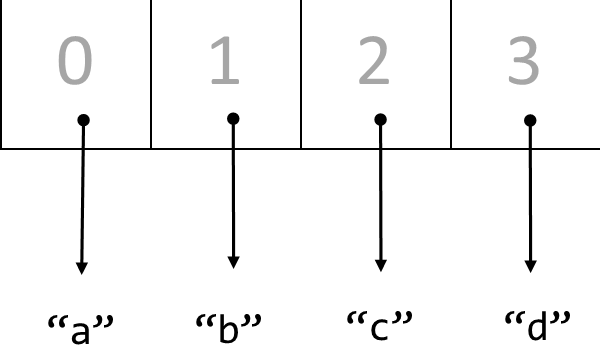
\includegraphics{diagrams/list-1}
  \end{center}
  \posttabularspace

  A list is similar to a frame. In a frame (list), a variable (index) is bound to a value (element), and you can retrieve the value (element) by using the variable (index). You can see that this list has four references, each of which points to one of the elements in a list. And, because this is a list, each reference has an integer index (0, 1, 2, or 3). You can use the index to access or assign a particular reference in the list.

  For brevity, this document uses syntax like \listfour{\strval{a}}{\strval{b}}{\strval{c}}{\strval{d}} to represent the list above in text.

\subsection{Constructor Expressions}

A constructor expression creates a new set, list, tuple, or dictionary.
Here are some constructor expressions:

\newcommand{\listonetwothree}{\listthree{1}{2}{3}}
\newcommand{\mydicttwo}{\dicttwo{\strval{a}}{1} {\strval{b}}{2}}

  \pretabularspace
  \begin{tabular}{l c l}
  \expr{[1, 2, 3]} & \Ra & A list with elements \val{1}, \val{2}, and
  \val{3}, in that order:  \\
  \setexpr{1, 2} & \Ra & A set with elements \val{1} and \val{2}:
  \settwo{\val{1}}{\val{2}} or equivalently \settwo{\val{2}}{\val{1}} \\
  \dictexpr{\stringexpr{a}:1, \stringexpr{b}:2} & \Ra & A dictionary in which \strval{a} maps to
  \val{1} and \strval{b} maps to \val{2}:
  \dicttwo{\strval{a}}{\val{1}} {\strval{b}}{\val{2}} \\
  & &  or equivalently \dicttwo{\strval{b}}{\val{2}} {\strval{a}}{\val{1}} \\
  \expr{(\stringexpr{hello}, 5)} & \Ra & A tuple with elements \strval{hello} and
  \val{5}, in that order: \tupletwo{\strval{hello}}{5} \\
  \end{tabular}
  \posttabularspace

  In general, a constructor expression has the form:

  \begin{description}
    \item[List] \expr{[\mvar{EXPR}, \mvar{EXPR}, ..., \mvar{EXPR}]}
    \item[Set] \setexpr{\mvar{EXPR}, \mvar{EXPR}, ..., \mvar{EXPR}}
    \item[Tuple] \expr{(\mvar{EXPR}, \mvar{EXPR}, ..., \mvar{EXPR})}
    \item[Dictionary] \dictexpr{\mvar{KEY\_EXPR}:\mvar{VAL\_EXPR}, ..., \mvar{KEY\_EXPR}:\mvar{VAL\_EXPR}}
  \end{description}

  A string constructor is a string literal such as \expr{"Hello world"}.

\subsubsection{Rules for Evaluation}

  To evaluate a constructor expression to a value, use these rules.

  \myparagraph{Lists, Sets, and Tuples}
  \begin{enumerate}
    \item
    From left to right, for each expression \mvar{EXPR} in the comma-separated
    list, evaluate \mvar{EXPR} to a value and replace \mvar{EXPR} with that
    value.

    \item
    Replace the constructor expression with a list, set, or tuple value containing
    exactly the values from the previous step. Retain order for a list or tuple.
    Remove duplicate elements for a set.

  \end{enumerate}

  \myparagraph{Dictionaries}
  \begin{enumerate}
    \item
    For each expression \expr{\mvar{KEY\_EXPR}:\mvar{VAL\_EXPR}} in the comma-separated list, from left to right, do the following:
    \begin{enumerate}
      \item
      Evaluate \mvar{VAL\_EXPR} to a value and replace \mvar{VAL\_EXPR} with that value.

      \item
      Evaluate \mvar{KEY\_EXPR} to a value and replace \mvar{KEY\_EXPR} with that value.

    \end{enumerate}

    \item
    Replace the constructor expression with a dictionary containing exactly the
    mappings from the previous step. If there are multiple mappings for a particular
    key, use the last (rightmost) mapping in the constructor expression.

  \end{enumerate}

\subsubsection{Examples}

  Below are examples of evaluating constructor expressions. Each example contains a constructor and a description of the data structure the constructor creates.

  \begin{enumerate}
    \item \expr{[0, 1, 0]} \\
    Creates a new list that contains the values \val{0}, \val{1}, and \val{0} at the indices 0, 1, and 2, respectively:
    \listthree{0}{1}{0}
    \item \expr{[]} \\
    Creates a new, empty list: \listzero
    \item \expr{(3.14159, \stringexpr{pi})} \\
    Creates a new two-tuple with the values \val{3.14159} and \strval{pi} at the indices 0 and 1, respectively:
    \tupletwo{3.14159}{\strval{pi}}
    \item \expr{(12,)} \\
    Creates a new 1-tuple with the value \val{12} at index 0:
    \tupleone{12}.  Note the trailing comma, which makes Python interpret
    the value inside the parentheses as a tuple rather than a parenthetical
    expression (as discussed in Section~\ref{compoundexpressions}).  A
    1-tuple isn't very useful (you may as well just use a single value), so
    you should avoid using them.
    \item \expr{()} \\
    Creates a new, empty tuple: \tuplezero\ .
    It's rarely useful to create a tuple with no elements.
    \item \dictexpr{\stringexpr{a}:1, \stringexpr{b}:2, \stringexpr{c}:3} \\
    Creates a new dictionary in which the key \strval{a} maps to the value \val{1}, \strval{b} maps to \val{2}, and \strval{c} maps to \val{3}:
    \dictthree{\strval{a}}{\val{2}} {\strval{b}}{\val{2}} {\strval{c}}{\val{3}}
    \item \dictexpr{\stringexpr{a}:1, \stringexpr{a}:0, \stringexpr{b}:2, \stringexpr{a}:3} \\
    Creates a new dictionary in which the key \strval{b} maps to the value \val{2} and \strval{a} maps to \val{3}. Note that the rightmost mapping for \strval{a} overwrites all previous mappings for that key:
    \dicttwo{\strval{b}}{\val{2}} {\strval{a}}{\val{3}}
    \item \dictexpr{\stringexpr{a}:1, \stringexpr{b}:1} \\
    Creates a new dictionary in which \strval{a} and \strval{b} both map to \val{1}. Note that although keys in a dictionary must be unique, the values need not be:
    \dicttwo{\strval{a}}{\val{1}} {\strval{b}}{\val{1}}
    \item \dictexpr{} \\
    Creates a new, empty dictionary: \dictzero
    \item \setexpr{0, 1, 2, 3} \\
    Creates a new set that contains the values \val{0}, \val{1}, \val{2}, and \val{3}:
    \setfour{\val{0}}{\val{1}}{\val{2}}{\val{3}}
    \item \setexpr{0, 1, 1, \stringexpr{hello}} \\
    Creates a new set that contains the values \val{0}, \val{1}, and \strval{hello}:
    \setthree{\val{0}}{\val{1}}{\strval{hello}}
    \item \expr{set()} \\
    Creates a new, empty set: \setzero. The expression \dictexpr{} creates an empty dictionary, not an empty set.
  \end{enumerate}

\subsection{Data Structure Access Expressions}
\label{datastructure-access}

Here are some examples of access expressions (accessing an element of a
data structure), the following variables are defined:

  \pretabularspace
  \begin{tabular}{l c l}
  \# \expr{lst} is \listonetwothree &  &  \\
  \# \expr{dict} is \dicttwo{\strval{a}}{\val{1}} {\strval{b}}{\val{2}} &  &  \\
  \end{tabular}
  \posttabularspace

  \pretabularspace
  \begin{tabular}{l c l}
  \expr{lst[0]} & \Ra & \val{1} \\
  \expr{lst[1]} & \Ra & \val{2} \\
  \expr{lst[-1]} & \Ra & \val{3} \\
  \expr{lst[-2]} & \Ra & \val{2} \\
  \expr{dict[\stringexpr{a}]} & \Ra & \val{1} \\
  \end{tabular}
  \posttabularspace

Sequences and dictionaries all provide methods for retrieving specific
values from the structure.  A dictionary access takes a key; the dictionary
access expression evaluates to the value associated with that key.  A
sequence access takes an index; the sequence access expression evaluates to
the element at that index.  The following sections describe how to evaluate
access expressions.  An access expression has the general form:

  \begin{description}
    \item \expr{\mvar{EXPR}[\mvar{INDEX\_EXPR}]}
  \end{description}

  Note that sets don't provide a way to access specific elements. If, in your code, you need to access a particular element in a set, then consider using a different data structure.

\subsubsection{Rules for Evaluation}

  \myparagraph{To evaluate \expr{\mvar{EXPR}[\mvar{INDEX\_EXPR}]} to a value}
  This expression returns a single value in the data structure given by \mvar{EXPR}.
  \begin{enumerate}
    \item
    Evaluate \mvar{EXPR} to a value and replace \mvar{EXPR} with that value.

    \item
    Evaluate \mvar{INDEX\_EXPR} to a value and replace \mvar{INDEX\_EXPR} with that value.

    \item
    If \mvar{EXPR} evaluates to something other than a sequence or dictionary, then raise an error.

    \item
    \begin{description}
      \item[If \mvar{EXPR} is a sequence] If \mvar{INDEX\_EXPR} is not an integer on the interval [$-n$, $n-1$] (inclusive, where $n$ is the length of the sequence), then this access fails.

      If \mvar{INDEX\_EXPR} is negative, replace \mvar{INDEX\_EXPR} with
      $n - \left|\mvar{INDEX\_EXPR}\right|$.  (Note that accessing index -1 is equivalent to accessing the last element in the sequence.)

      Replace the access expression with the value in the sequence at that index. Sequences are zero-indexed, so the first value in the sequence is at index 0.

      \item[If \mvar{EXPR} is a dictionary] The expression succeeds only if \mvar{INDEX\_EXPR} is a key in the dictionary. Replace the entire access expression with the value to which the key maps.
    \end{description}
  \end{enumerate}

\subsubsection{Examples}

  Below are examples of evaluating access expressions. Each example
  contains an access expression and the value to which that access
  evaluates.

Each example is executed in the context of this frame, unaffected by previous examples:

\newcommand{\mylist}{\listfour{0}{5}{3}{4}}
\newcommand{\mydict}{\dictthree{\strval{a}}{1} {\strval{b}}{2} {\strval{c}}{\strval{a}}}
\newcommand{\mytuple}{\tupletwo{\strval{hello}}{5}}

  \begin{itemize}
    \item \expr{mylist} is \mylist
    \item \expr{mydict} is \mydict
    \item \expr{mytuple} is \mytuple
  \end{itemize}

  \begin{enumerate}
    \item
      \expr{\ul{mylist}[0]} \\
      \expr{\mylist[\ul{0}]} \\
      \expr{\ul{\mylist[\val{0}]}} \\
      \val{0}

    \item \expr{mylist[4]} \\
    ERROR. No index 4.

    \item \expr{mylist[3]} \\
    \val{4}

    \item
      \expr{\ul{mylist}[-1]} \\
      \expr{\mylist[\ul{-1}]} \\
      \expr{\mylist[\ul{len(mylist)}-1]} \\
      \expr{\mylist[\ul{\val{4}-\val{1}}]} \\
      \expr{\ul{\mylist[\val{3}]}} \\
      \val{4}

    \item
      \expr{\ul{mylist}[0 - 3]} \\
      \expr{\mylist[\ul{0 - 3}]} \\
      \expr{\mylist[\ul{\val{-3}}]} \\
      \expr{\mylist[\ul{len(mylist)}-\val{3}]} \\
      \expr{\mylist[\ul{\val{4}-\val{3}}]} \\
      \expr{\ul{\mylist[\val{1}]}} \\
      \val{5}

    \item
      \expr{\ul{mydict}[\stringexpr{a}]} \\
      \expr{\mydict[\ul{\stringexpr{a}}]} \\
      \expr{\ul{\mydict[\strval{a}]}} \\
      \val{1}

    \item
      \expr{mydict[mydict[\ul{\stringexpr{c}}]]} \\
      \expr{mydict[\ul{mydict[\strval{c}]}]} \\
      \expr{\ul{mydict[\strval{a}]}} \\
      \val{1}

      We skipped evaluating \expr{mydict} to {\mydict} in this example, for
      brevity.


    \item \expr{mydict[(12, 13)]} \\
    ERROR. The value \tupletwo{12}{13} is not a key in the dictionary.

    \item
      \expr{\ul{mytuple}[0]} \\
      \expr{\mytuple[\ul{0}]} \\
      \expr{\mytuple[\val{0}]} \\
      \strval{hello}

    \item \expr{mytuple[1]} \\
    \val{5}

    \item
      \expr{\ul{mytuple}[-1]} \\
      \expr{\mytuple[\ul{-1}]} \\
      \expr{\mytuple[\ul{\val{-1}}]} \\
      \expr{\mytuple[\ul{len(mytuple)}-\val{1}]} \\
      \expr{\mytuple[\ul{\val{2}-\val{1}}]} \\
      \expr{\ul{mytuple[\val{1}]}} \\
      \val{5}
  \end{enumerate}

\subsection{Data Structure Assignment Statements}
\label{data-structure-assignment-statements}

  In the same way that sequences and dictionaries provide a way to access individual elements, they also provide a way to reassign individual elements. This lets you change the elements of the structure. Here are some examples of reassigning an element of a data structure:

  \pretabularspace
  \begin{tabular}{l l}
  \# \expr{lst} is \listonetwothree &  \\
  \# \expr{dict} is \dicttwo{\strval{a}}{\val{1}} {\strval{b}}{\val{2}} &  \\
  \end{tabular}
  \posttabularspace

  \pretabularspace
  \begin{tabular}{l l}
  \expr{lst[0] = 17} & after this, \expr{lst} is \listthree{\val{17}}{\val{2}}{\val{3}} \\
  \expr{lst[-1] = 18} & after this, \expr{lst} is \listthree{\val{1}}{\val{2}}{\val{18}} \\
  \expr{dict[\stringexpr{b}] = 12} & after this, \expr{dict} is \dicttwo{\strval{a}}{\val{1}} {\strval{b}}{\val{12}} \\
  \end{tabular}
  \posttabularspace

  In general, an element assignment statement has the form:

% "DS_EXPR" probably stands for "data structure expression".

  \begin{description}
    \item \expr{\mvar{DS\_EXPR}[\mvar{EXPR}] = \mvar{ASSIGN\_EXPR}}
  \end{description}

Element assignments are very similar to variable assignments.  There is an
l-expression (on the \textbf{l}eft of the assignment operator; the the
example above, it is \expr{\mvar{DS\_EXPR}[\mvar{EXPR}]}) and an r-expression
(on the \textbf{r}ight; in the example, it is \expr{\mvar{ASSIGN\_EXPR}}).
The l-expression is not evaluated to a value; rather, it
identifies a particular reference or binding in the structure.   The
assignment makes that reference point to the value to which r-expression
evaluates.

Tuples and sets don't provide a way to reassign specific values.  It isn't
surprising that sets don't support this operation, because sets don't even
provide a way to access specific values.  Tuples, on the other hand, do not
support this operation because they are immutable: once created, they cannot
change.

\subsubsection{Rules for Evaluation}

  Assigning a single element makes that particular reference point to a different value. To execute an element assignment statement,

  \begin{enumerate}
    \item
    Evaluate the r-expression to a value and replace the r-expression with that value.

  \item
    Evaluate the l-expression to identify a particular reference in the
    data structure.  When accessing a single index in a list, this
    statement will fail if the index is not in the list.  However, when
    accessing a key in a dictionary, if the key is not in the dictionary
    already then Python will add it and the l-expression will identify a
    reference for this new key.

    \item
    Change the reference so that it points to the value given by the r-expression.
  \end{enumerate}

\subsubsection{Examples}

  Below are examples of executing assignment statements. Each example contains an assignment statement, some intermediate steps of executing the statement shown underneath, and the final value of the affected data structure.

Each example is executed in the context of this frame, unaffected by previous examples:

  \begin{itemize}
    \item \expr{lst} is \listonetwothree
    \item \expr{dict} is \mydicttwo
    \item \expr{t} is \tupletwo{\strval{hello}}{5}
  \end{itemize}

  % In Python:
  % lst = [1,2,3]
  % dict = {"a":1,"b":2}
  % t = ("hello", 5)

  \begin{enumerate}
    \item
      \expr{lst[0] = \ul{17}} \\
      \expr{\ul{lst}[0] = \val{17}} \\
      \expr{\listonetwothree[\ul{0}] = \val{17}} \\
      \ul{\expr{\listonetwothree[\val{0}] = \val{17}}} \\
      Now, \expr{lst} \Ra \listthree{17}{2}{3}.

      Note that in this example we did not evaluate the l-value
      \expr{lst[0]} to a value; rather, we evaluated the parts and then
      used them to assign one of the slots of \expr{lst}.

    \item
      \expr{dict[lst[0]] = \ul{\stringexpr{c}}} \\
      \expr{\ul{dict}[lst[0]] = \strval{c}} \\
      \expr{\mydicttwo[\ul{lst[0]}] = \strval{c}} \\
      \ul{\expr{\mydicttwo[\val{1}] = \strval{c}}} \\
      Now, \expr{dict} \Ra \dictthree{\strval{a}}{2} {\strval{b}}{2} {1}{\strval{c}}.

    \item \expr{dict[\stringexpr{a}] = lst[1]} \\
      \vdots \\
    \expr{\mydicttwo[\strval{a}]} = \val{2} \\
    Now, \expr{dict} \Ra \dicttwo{\strval{a}}{2} {\strval{b}}{2}.

    \item \expr{t[1] = 6} \\
    ERROR: `tuple' object does not support item assignment. \\
    (That is Python's way of saying that \expr{t}'s value is immutable.)

    \item \expr{dict[\stringexpr{a}] = lst} \\
    % TODO: show this in a real frame diagram.
    Now, \expr{dict} \Ra \dicttwo{\strval{a}}{\listonetwothree} {\strval{b}}{2} where \listonetwothree is the same list value as \expr{lst} has
  \end{enumerate}

\subsection{Sequence Slice Access and Assignment Expressions}

Just as a list access evaluates to a single element of the list, a slice
operation evaluates to multiple elements of the list --- that is, a
subsequence.
You can also assign to a slice, which modifies the original sequence by
adding or replacing a sequence of elements. Here are some examples of slice
accesses and assignments.

  \pretabularspace
  \begin{tabular}{l c l}
  \# \expr{lst} is \listonetwothree &  \\
  \expr{lst[0:2]} & \Ra & \listtwo{1}{2} \\
  \expr{lst[0:2] = [\stringexpr{a}, \stringexpr{b}, \stringexpr{c}]} & after this, \expr{lst} is \listfour{\strval{a}}{\strval{b}}{\strval{c}}{\val{3}} \\
  \end{tabular}
  \posttabularspace

  In general, a list slice access expression has the form:

  \begin{description}
    \item \expr{\mvar{EXPR}[\mvar{INDEX\_EXPR\_1}:\mvar{INDEX\_EXPR\_2}]}
  \end{description}

  In general, a list slice assignment expression has the form:

  \begin{description}
    \item \expr{\mvar{DS\_EXPR}[\mvar{INDEX\_EXPR\_1}:\mvar{INDEX\_EXPR\_2}] = \mvar{ASSIGN\_EXPR}}
  \end{description}

  The rules for evaluating a slice operation have many special cases, which makes debugging slices very difficult. For this reason, you should avoid using slices for anything but the most predictable operations.

\subsubsection{Rules for Evaluation}

  \myparagraph{To evaluate \expr{\mvar{EXPR}[\mvar{INDEX\_EXPR\_1}:\mvar{INDEX\_EXPR\_2}]} to a value}
  \begin{enumerate}
    \item
    Evaluate \mvar{EXPR} to a value and replace \mvar{EXPR} with that value. \\
    Henceforth in these rules, mentions of \mvar{EXPR} mean the value,
    not the original expression.

    \item
    If the expression has any of the following forms, transform it as
    described below.  These Python shorthands make it easy for a programmer
    to select the first or last few elements of the sequence.
    \begin{description}
      \item[\expr{\mvar{EXPR}[:\mvar{INDEX\_EXPR\_2}]}] becomes \expr{\mvar{EXPR}[0:\mvar{INDEX\_EXPR\_2}]}
      \item[\expr{\mvar{EXPR}[\mvar{INDEX\_EXPR\_1}:]}] becomes \expr{\mvar{EXPR}[\mvar{INDEX\_EXPR\_1}:len(\mvar{EXPR})]}
      \item[\expr{\mvar{EXPR}[:]}] becomes \expr{\mvar{EXPR}[0:len(\mvar{EXPR})]}
    \end{description}

    \item
    Evaluate \mvar{INDEX\_EXPR\_1} to a value and replace the expression with that value. Then do the same for \mvar{INDEX\_EXPR\_2}.

    \item
    Let $n$ be the length of \mvar{EXPR}.
    If either index is less than $-n$, replace it with $-n$. If either index is greater than $n$, replace it with $n$.

    \item
    Let $n$ be the length of \mvar{EXPR}.
    If \mvar{INDEX\_EXPR\_1} is negative, replace it with $n - \left|\mvar{INDEX\_EXPR\_1}\right|$.
    Then do the same for \mvar{INDEX\_EXPR\_2}. At this point, both indices should be on the interval $[0, n]$ (note that $n$ is a valid index in a slice, but not in an access to a single element).

    \item
    Raise an error if \mvar{EXPR} is not a sequence.

    \item
      Let $i$ be the first index value, and let $j$ be the second.  Create
      a list of indices containing every integer $x$ such that $i \le x <
      j$.  (For example, if $i$ is 2 and $j$ is 4, then this list will
      contain 2 and 3.)  Note that it is possible for this list to be empty
      (for instance, if $j \le i$).

    \item
    For each $x$ in this list of indices, replace $x$ with the value in the
    original sequence at index $x$.  Replace the slice access with this new
    list.  It is important to note that the slice returns a new list, so
    reassigning elements of the slice does not affect the original list.
  \end{enumerate}

  Reassigning a slice first removes that slice, then inserts a new sequence of references starting at the lowest index of the slice.

  \myparagraph{To execute \expr{\mvar{DS\_EXPR}[\mvar{INDEX\_EXPR\_1}:\mvar{INDEX\_EXPR\_2}] = \mvar{ASSIGN\_EXPR}}}
  \begin{enumerate}
    \item
    Evaluate the r-expression \mvar{ASSIGN\_EXPR} to a value and replace
    \mvar{ASSIGN\_EXPR} by that value.

    \item
    Evaluate the l-expression to identify a sequence of l-references in the data structure.

    \item
    Raise an error if (a) \mvar{DS\_EXPR} is not a sequence, or (b) the r-expression is not another data structure.

    \item
    Remove the specified slice from the original sequence (if the slice is empty, don't remove anything).

    \item
    Create a new list containing the elements of \mvar{ASSIGN\_EXPR} in iterator order.

    \item
    Insert, starting at the lowest index in the slice, the sequence of references in the list from the previous step.
  \end{enumerate}

\subsubsection{Examples}

In these examples, \expr{mylist} is \mylist.


  \begin{enumerate}
    \item \expr{mylist[0:3]} \\
    indices 0, 1, and 2 \\
    \listthree{0}{5}{3}

    \item \expr{mylist[-3:0]} \\
    \expr{mylist[\val{1}:\val{0}]} \\
    no indices \\
    \listzero

    \item \expr{mylist[-100:100]} \\
    \expr{mylist[\val{-4}:\val{4}]} \\
    \expr{mylist[\val{0}:\val{4}]} \\
    indices 0, 1, 2, and 3 \\
    \listfour{0}{5}{3}{4}

    \item \expr{mylist[1:]} \\
    \expr{mylist[\val{1}:len(mylist)]} \\
    \expr{mylist[\val{1}:\val{4}]} \\
    indices 1, 2, and 3 \\
    \listthree{5}{3}{4}

    \item \expr{mylist[-3:]} \\
    \expr{mylist[\val{-3}:len(mylist)]} \\
    \expr{mylist[\val{-3}:\val{4}]} \\
    \expr{mylist[\val{1}:\val{4}]} \\
    indices 1, 2, and 3 \\
    \listthree{5}{3}{4}

    \item \expr{mylist[:]} \\
    \expr{mylist[\val{0}:len(mylist)]} \\
    \expr{mylist[\val{0}:\val{4}]} \\
    indices 0, 1, 2, and 3 \\
    \listfour{0}{5}{4}{3}

    \item \expr{mylist[0:3] = [\stringexpr{hello}, \stringexpr{there}}] \\
    indices to replace: 0, 1, and 2 \\
    list to insert: \listtwo{\strval{hello}}{\strval{there}} \\
    \listthree{\strval{hello}}{\strval{there}}{3}

    \item \expr{mylist[0:3] = \setexpr{\stringexpr{hello}, \stringexpr{there}}} \\
    indices to replace: 0, 1, and 2 \\
    list to insert: \listtwo{\strval{hello}}{\strval{there}}
    \emph{or} \listtwo{\strval{there}}{\strval{hello}}; Python will choose
    one of these arbitrarily because the argument is a set, which does not
    have a defined order. \\
    \listthree{\strval{hello}}{\strval{there}}{3}
    \emph{or} \listthree{\strval{there}}{\strval{hello}}{3}

    \item \expr{mylist[:1] = [\stringexpr{a}, \stringexpr{b}]} \\
    \expr{mylist[0:1] = [\stringexpr{a}, \stringexpr{b}]} \\
    indices to replace: 0 \\
    list to insert: \listtwo{\strval{a}}{\strval{b}} \\
    \listfive{\strval{a}}{\strval{b}}{5}{3}{4}

    \item \expr{mylist[:] = [\stringexpr{b}, \stringexpr{c}]} \\
    \expr{mylist[0:len(mylist)] = [\stringexpr{b}, \stringexpr{c}]} \\
    \expr{mylist[\val{0}:\val{4}] = [\stringexpr{b}, \stringexpr{c}]} \\
    indices to replace: 0, 1, 2, and 3 \\
    list to insert: \listtwo{\strval{b}}{\strval{c}} \\
    \listtwo{\strval{b}}{\strval{c}}
  \end{enumerate}


\subsection{\kw{del} Statements}

  The \kw{del} keyword removes elements from lists and dictionaries. Here are some example statements that use the \kw{del} keyword:

  \pretabularspace
  \begin{tabular}{l l}
  \expr{\# lst = [1, 2, 3, 4]} &  \\
  \expr{\# d = {\stringexpr{a}:1, \stringexpr{b}:2}} &  \\
  \expr{del lst[0]} & \expr{\# lst is [2, 3, 4]}  \\
  \expr{del lst[0:2]} & \expr{\# lst is [3, 4]} \\
  \expr{del d[\stringexpr{a}]} & \expr{\# d is \{\stringexpr{b}:2\}} \\
  \end{tabular}
  \posttabularspace

  In general, a \kw{del} statement has the form:

  \begin{description}
    \item \expr{del \mvar{ACCESS\_EXPR}}
    \item \expr{del \mvar{ACCESS\_EXPR}, \mvar{ACCESS\_EXPR}}
  \end{description}

\subsubsection{Rules for Evaluation}

  \myparagraph{To execute \expr{del \mvar{ACCESS\_EXPR}}}
  \begin{enumerate}
    \item
    Perform a data structure access on \mvar{ACCESS\_EXPR}. The \kw{del} statement fails if the access is not to a list or dictionary.

    \item
    Choose one of the following:
    \begin{description}
      \item[If \mvar{DS\_EXPR} is a list] The access refers to particular element (or slice) of the list. Remove this element (slice) from the list.
      \item[If \mvar{DS\_EXPR} is a dictionary] The access refers to a key-value mapping in the dictionary. Remove this binding from the dictionary.
    \end{description}

  \end{enumerate}

  \myparagraph{To execute \expr{del \mvar{ACCESS\_EXPR}, \mvar{ACCESS\_EXPR}, ...}}
  This statement lets you delete several items in a single line of code.
  Convert it into a sequence of single-element \expr{del} statements.

%  Note that if any deletion fails and raises an error, none of the following deletions will execute, but the effects of previous deletions will remain.
%   \begin{enumerate}
%     \item
%     Let the current expression be the leftmost \mvar{ACCESS\_EXPR}.
%
%     \item
%     Execute a \kw{del} statement on the current expression.
%
%     \item
%     Let the current expression be the next expression (directly to the right of the current expression), then go to the previous step. If no such expression exists, stop executing.
%
%   \end{enumerate}

\subsubsection{Examples}

  Below are examples of executing \kw{del} statements. Each example contains a \kw{del} statement and the final value of the affected data structure(s). In the following examples, the following variables are defined.

Each example starts with these variables defined, unaffected by previous examples.

  \begin{itemize}
    \item \expr{lst4} is \listfour{0}{1}{2}{3}
    \item \expr{dict} is \mydicttwo
  \end{itemize}

  % For Python repl:
  % lst4 = [0, 1, 2, 3]
  % dict = {'a':1, 'b':2}

  \begin{enumerate}
    \item \expr{del lst4[0]} \\
    \listonetwothree

    \item \expr{del lst4[-1]} \\
    \listthree{0}{1}{2}

    \item \expr{del lst4[:]} \\
    \listzero

    \item \expr{del lst4[0:2]} \\
    \listtwo{2}{3}

    \item \expr{del dict[\stringexpr{a}]} \\
    \dictone{\strval{b}}{2}

    \item \expr{del dict[\stringexpr{c}]} \\
    ERROR. KeyError (\stringexpr{c} is not a key in dict)

    \item \expr{del dict[\stringexpr{a}], dict[\stringexpr{c}]}  \\
    First deletes \expr{dict[\stringexpr{a}]}, then throws an error on \expr{dict[\stringexpr{c}]}. At the end, \expr{dict} is \dictone{\strval{b}}{2}

    \item \expr{del lst4[0], dict[{\stringexpr{b}}]} \\
    \expr{lst4} is \listthree{1}{2}{3} and \expr{dict} is \dictone{\strval{a}}{1}
  \end{enumerate}


%% TODO: write this section
% \subsection{Multiple Assignment Statements (also known as Parallel, Tuple,
%   or Structured Assignments)}}
% 
% It is permitted 
% 
% \subsubsection{Rules for Evaluation}
% 
% \subsubsection{Examples}


\section{Loop Statements}
\label{sec:loop-statements}
\subsection{\kw{for} Loop Statements}

A \kw{for} loop executes its body multiple times.  The \kw{for} loop
\emph{iterates} over a sequence such as a list or string, and executes the
body once for each element in the sequence.
A \kw{for} loop also defines a loop variable.  On each
iteration, the loop variable is assigned to the next sequence element.
Here is an example of a \kw{for} loop:

\begin{verbatim}
  for value in [1, 2, 6]:
      print value + 1
\end{verbatim}

  This code prints:
\begin{verbatim}
  2
  3
  7
\end{verbatim}

  In general, a \kw{for} loop has the form:

  \pretabularspace
  \noindent \expr{for \mvar{LOOP\_VAR} in \mvar{DS\_EXPR}:} \\
  \indent \mvar{BODY\_STATEMENTS}
  \posttabularspace

\subsubsection{Rules for Evaluation}
\label{sec:loop-evaluation-rules}

We give two rules for evaluating \kw{for} loop:  a control-oriented
version, and a rewriting version.  They produce identical results, and you
can use whichever one you prefer.



  To execute a \kw{for} loop,

  \begin{enumerate}
    \item
    Evaluate \mvar{DS\_EXPR} to a value and replace the expression with that value.

    \item
    Assign the \mvar{LOOP\_VAR} to the first value in the sequence. If the sequence is empty (contains no elements), exit the loop.

    \item
    Execute the statements in the body of the loop.  If you encounter a
    \kw{break} statement, immediately exit the loop.  If you encounter a
    \kw{continue} statement, immediately continue to the next step.
    For more information, see Section~\ref{sec:break-statement} on the
    \kw{break} statement and Section~\ref{sec:continue-statement} on the
    \kw{continue} statement.

    \item
    Reassign \mvar{LOOP\_VAR} to the next value in the sequence, then
    repeat the previous step.  If there is no next element, exit the
    loop.  For lists, the next element is the element at the next index.  For
    sets and dictionaries, the order is undefined, so the next element can
    be any of the remaining elements.

  \end{enumerate}

  You can also evaluate a loop by rewriting it.  Rewriting a loop is too
  cumbersome to use regularly, but it's unambiguous and therefore can yield
  insight.  To rewrite a \kw{for} loop,

  \begin{enumerate}
    \item
    Evaluate the \mvar{DS\_EXPR} to a value.

    \item
    Write an assignment to the loop variable for each element in \mvar{DS\_EXPR} (if the data structure is a sequence such as a list, make sure the assignments are in the same order as in the list). For example, if the sequence had four elements, you would write four assignments.

    \item
    Write a copy of the loop's body after each assignment.

    \item
    Execute the resultant statements. \\
    If you encounter a \kw{break}
    statement, immediately skip to the end of the loop statements by
    deleting them all --- that is, rewriting them to nothing. \\
    If you
    encounter a \kw{continue} statement, immediately skip to the next
    assignment of the loop variable \mvar{LOOP\_VAR} by deleting all
    statements up to that point --- that is, rewriting them to nothing. \\
    For more information, see Section~\ref{sec:break-statement} on the
    \kw{break} statement and Section~\ref{sec:continue-statement} on the
    \kw{continue} statement.

  \end{enumerate}

\subsubsection{Examples}

Below are examples of executing \kw{for} loops, using the rewriting
approach.  Each example contains a \kw{for} loop and a sequence of
assignments to the loop variable in the correct order.  (For sets and
dictionaries, remember that the order is undefined.)

  \begin{enumerate}
    \item
    \begin{enumerate}
      \item
\begin{verbatim}
for y in ['hello', 'there', 'hi']:
  BODY_STATEMENTS
\end{verbatim}
      \item
\begin{verbatim}
y = 'hello'
BODY_STATEMENTS
y = 'there'
BODY_STATEMENTS
y = 'hi'
BODY_STATEMENTS
\end{verbatim}
    \end{enumerate}

    \item
    \begin{enumerate}
      \item
\begin{verbatim}
for x in [17, 12, 14, 13, 14, 18]:
  BODY_STATEMENTS
\end{verbatim}
      \item
\begin{verbatim}
x = 17
BODY_STATEMENTS
x = 12
BODY_STATEMENTS
x = 14
BODY_STATEMENTS
x = 13
BODY_STATEMENTS
x = 14
BODY_STATEMENTS
x = 18
BODY_STATEMENTS
\end{verbatim}
    \end{enumerate}

    \item
    \begin{enumerate}
      \item
\begin{verbatim}
for x in [1, 3]:
  for y in [2, 4]:
    BODY_STATEMENTS
\end{verbatim}
      \item
\begin{verbatim}
x = 1
y = 2
BODY_STATEMENTS
y = 4
BODY_STATEMENTS
x = 3
y = 2
BODY_STATEMENTS
y = 4
BODY_STATEMENTS
\end{verbatim}
    \end{enumerate}

    \item
    \begin{enumerate}
      \item
\begin{verbatim}
for x in [1, 1, 3]:
  BODY_STATEMENTS_1
  for y in {'a', 'b', 'c'}:
    BODY_STATEMENTS_2
\end{verbatim}
      \item
\begin{verbatim}
x = 1
BODY_STATEMENTS_1
y = 'a'
BODY_STATEMENTS_2
y = 'b'
BODY_STATEMENTS_2
y = 'c'
BODY_STATEMENTS_2
x = 1
BODY_STATEMENTS_1
y = 'a'
BODY_STATEMENTS_2
y = 'b'
BODY_STATEMENTS_2
y = 'c'
BODY_STATEMENTS_2
x = 3
BODY_STATEMENTS_1
y = 'a'
BODY_STATEMENTS_2
y = 'b'
BODY_STATEMENTS_2
y = 'c'
BODY_STATEMENTS_2
\end{verbatim}
    \end{enumerate}

%% Todo: reinstate once the rules describe multiple/tuple/parallel assignment.
%     \item
%     \begin{enumerate}
%       \item
% \begin{verbatim}
% for (x, y) in [('hello', 5), ('this', 4)]:
%   BODY_STATEMENTS_1
%   for z in [10, 15]:
%     BODY_STATEMENTS_2
% \end{verbatim}
%       \item
% \begin{verbatim}
% (x, y) = ('hello', 5)
% BODY_STATEMENTS_1
% z = 10
% BODY_STATEMENTS_2
% z = 15
% BODY_STATEMENTS_2
% (x, y) = ('this', 4)
% BODY_STATEMENTS_1
% z = 10
% BODY_STATEMENTS_2
% z = 15
% BODY_STATEMENTS_2
% \end{verbatim}
%     \end{enumerate}

    \item
    \begin{enumerate}
      \item
\begin{verbatim}
for x in [15, 10, 12, 13, 17, 14, 16]:
  if x >= 15:
    for y in ['a', 'b']:
      BODY_STATEMENTS_1
  BODY_STATEMENTS_2
\end{verbatim}
      \item
\begin{verbatim}
x = 15
if x >= 15:
  for y in ['a', 'b']:
    BODY_STATEMENTS_1
BODY_STATEMENTS_2
x = 10
if x >= 15:
  for y in ['a', 'b']:
    BODY_STATEMENTS_1
BODY_STATEMENTS_2
x = 12
if x >= 15:
  for y in ['a', 'b']:
    BODY_STATEMENTS_1
BODY_STATEMENTS_2
x = 13
if x >= 15:
  for y in ['a', 'b']:
    BODY_STATEMENTS_1
BODY_STATEMENTS_2
x = 17
if x >= 15:
  for y in ['a', 'b']:
    BODY_STATEMENTS_1
BODY_STATEMENTS_2
x = 14
if x >= 15:
  for y in ['a', 'b']:
    BODY_STATEMENTS_1
BODY_STATEMENTS_2
x = 16
if x >= 15:
  for y in ['a', 'b']:
    BODY_STATEMENTS_1
BODY_STATEMENTS_2
\end{verbatim}
    \end{enumerate}

    \item
    \begin{enumerate}
      \item
%% Alternate Yoda quates:
% Strong you are with the dark side
% Mysterious are the ways of the Force.
\begin{verbatim}
for x in {'you', 'will', 'consume', 'it'}:
  BODY_STATEMENTS
\end{verbatim}
      \item
\begin{verbatim}
x = 'consume'
BODY_STATEMENTS
x = 'you'
BODY_STATEMENTS
x = 'it'
BODY_STATEMENTS
x = 'will'
BODY_STATEMENTS
\end{verbatim}
    \end{enumerate}

  \end{enumerate}

\subsection{\kw{while} Loop Statements}

A \kw{while} loop is like a \kw{for} loop in that it executes a block of
statements repeatedly.  However, whereas a \kw{for} loop executes exactly
one time for each element in a data structure, a \kw{while} loop executes
an indefinite number of times while a condition is \val{True} (or,
conversely, until a condition is \val{False}).  Here's an example of a
\kw{while} loop that computes \expr{x} to the power \expr{y}, or
$\expr{x}^\expr{y}$:

\begin{verbatim}
  # Computes x**y
  result = 1
  while y > 0:
      result = result * x
      y = y - 1
  # result = x**y
\end{verbatim}

  A \kw{while} loop has the general form below. Every \kw{while} loop includes a Boolean condition and some statements in its body.

  \pretabularspace
  \noindent \expr{while \mvar{BOOL\_EXPR}:} \\
  \indent \mvar{BODY\_STATEMENTS}
  \posttabularspace

  The \kw{while} loop can be confusing at first. It is easy to think that the loop exits the instant the condition becomes false, even if that happens in the middle of the loop, but this is not true. The condition is only checked once per iteration, at the beginning of that iteration, and if the condition is true then the entire body executes before the condition is checked again.

  To prevent this confusion, you should think of a \kw{while} loop as an if statement that repeats over and over again. That is, if the condition is true, then execute the body. If the condition is still true, execute the body, and so on until the condition is not true.

\subsubsection{Rules for Evaluation}

  To execute a \kw{while} loop,

  \begin{enumerate}
    \item
    Evaluate the condition of the loop.
        If the condition evaluates to a non-Boolean value,
        \linktotruthvaluetesting{convert the value to a Boolean value} (see
        \url{https://docs.python.org/2/library/stdtypes.html\#truth-value-testing}).
    If the value is \val{False}, exit the loop.

    \item
    Execute the entire body of the loop.
    After executing the entire body, go to the previous step.
    If you encounter a
    \kw{break} statement, immediately exit the loop.  If you encounter a
    \kw{continue} statement, immediately continue to the next step.
    For more information, see Section~\ref{sec:break-statement} on the
    \kw{break} statement and Section~\ref{sec:continue-statement} on the
    \kw{continue} statement.

  \end{enumerate}

  (It is possible to give a rewriting semantics for loops, similarly to how
  Section~\ref{sec:loop-evaluation-rules} gives both a control-oriented and
  a rewriting version of \kw{for} loop semantics.  We omit the rewriting
  semantics for \kw{while} loops, for brevity.)


\subsubsection{Examples}

  Below are examples of executing \kw{while} loops. Each example contains a \kw{while} loop, the values of several variables before the loop, and each variable's value after each iteration of the loop.

  \begin{enumerate}
    \item
    \begin{enumerate}
      \item
\begin{verbatim}
# lst = [1, 3, 2], i = 0
while i < len(lst):
   val = lst[i]
   i += 1
\end{verbatim}
      \item
After iteration 1: \\
\texttt{lst = [1, 3, 2], i = 1, val = 1} \\
After iteration 2: \\
\texttt{lst = [1, 3, 2], i = 2, val = 3} \\
After iteration 3: \\
\texttt{lst = [1, 3, 2], i = 3, val = 2}
    \end{enumerate}

    \item
    \begin{enumerate}
      \item
\begin{verbatim}
# result = 1, x = 2, y = 3
while y > 0:
    result = result * x
    y = y - 1
\end{verbatim}
      \item
After iteration 1: \\
\texttt{result = 2, x = 2, y = 2} \\
After iteration 2: \\
\texttt{result = 4, x = 2, y = 1} \\
After iteration 3: \\
\texttt{result = 8, x = 2, y = 0}
      \item Now, \expr{result} is $2^3$.  The original values of \expr{x}
        and \expr{y} were \val{2} and \val{3}.
    \end{enumerate}

    \item
    \begin{enumerate}
      \item
\begin{verbatim}
# fact = 1, i = 1
while i <= 4:
  i += 1
  fact *= i
\end{verbatim}
      \item
After iteration 1: \\
\texttt{fact = 2, i = 2} \\
After iteration 2: \\
\texttt{fact = 6, i = 3} \\
After iteration 3: \\
\texttt{fact = 24, i = 4}
After iteration 4: \\
\texttt{fact = 120, i = 5}
      \item After each iteration, \expr{fact} is \expr{i}!, the factorial of \expr{i}.
    \end{enumerate}
  \end{enumerate}

\subsection{\kw{break} Statements}
\label{sec:break-statement}

  The \kw{break} statement only appears inside the body of a \kw{for} or \kw{while} loop. Executing a \kw{break} statement immediately ends execution of the loop inside which it's declared. Here's an example of a \kw{break} statement:

\begin{verbatim}
  # s is a string
  i = 0
  for char in s:
    if char == ' ':
      break
    i += 1
  # i is the index of the first space in s
\end{verbatim}

  The \kw{break} keyword always appears on its own line, with no other expressions on the line.

\subsubsection{Rules for Evaluation}

  To execute a \kw{break} statement, immediately end execution of the loop. Do not execute any more lines in the body of the loop.

  If the \kw{break} statement is enclosed in a nested loop, only end execution of the innermost loop that contains the \kw{break} statement.

\subsubsection{Examples}

  Below are examples of executing \kw{break} statements. Each example contains a loop that contains a \kw{break} statement, and is formatted in the same style as in previous sections.

  \begin{enumerate}
    \item
    \begin{enumerate}
      \item
\begin{verbatim}
# i = 0, s = 'hello there'
for char in s:
  if char == ' ':
    break
  i += 1
\end{verbatim}
      \item
\begin{verbatim}
char = 'h'
i = 1
char = 'e'
i = 2
char = 'l'
i = 3
char = 'l'
i = 4
char = 'o'
i = 5
char = ' '
\end{verbatim}
      \item Note that \expr{i} is the index of the first space in \expr{s}.
    \end{enumerate}

    \item
    \begin{enumerate}
      \item
\begin{verbatim}
for x in [1, 2]:
  for y in ['a', 'b', 'c']:
    if y == 'b':
      break
\end{verbatim}
      \item
\begin{verbatim}
x = 1
y = 'a'
y = 'b'
x = 2
y = 'a'
y = 'b'
\end{verbatim}
    \end{enumerate}
  \end{enumerate}

\subsection{\kw{continue} Statements}
\label{sec:continue-statement}

  The \kw{continue} statement only appears inside the body of a \kw{for} or \kw{while} loop. Executing a \kw{continue} statement immediately ends execution of the current iteration of the loop and skips to the next iteration (as opposed to a \kw{break} statement, which exits the loop completely). Here is an example of a \kw{continue} statement:

\begin{verbatim}
  # lst is a list
  other = []
  for val in lst:
    if val is None:
      continue
    other.append(val)
  # other contains all the values in lst that are not None
\end{verbatim}

  Like the \kw{break} keyword, the \kw{continue} keyword always appears on its own line, with no other expressions on the line. Note that in general, it is bad style to use \kw{continue} because it is difficult to reason about.

\subsubsection{Rules for Evaluation}

  To execute a \kw{continue} statement, immediately move execution to the next iteration of the loop. Do not execute any more statements in the body of the loop for this iteration.

  For a \kw{while} loop, make sure to test the condition before starting the next iteration, and for a \kw{for} loop, remember to reassign the loop variable.

  Like the \kw{break} statement, if the \kw{continue} statement is enclosed in a nested loop, only skip to the next iteration of the innermost loop that contains the \kw{continue} statement.

\subsubsection{Examples}

  Below are examples of executing \kw{continue} statements. Each example contains a loop that contains a \kw{continue} statement, and is formatted in the same style as in previous sections.

\begin{verbatim}
  # Loop
  # lst = [1, None, None, 4], i = 0
  for val in lst:
    if val is None:
      continue
    i += 1

  # Assignments
  val = 1
  i = 1
  val = None
  val = None
  val = 4
  i = 2

  # Note that i is the number of values in lst that are not None
\end{verbatim}



\subsection{Comprehension Expressions}

  A comprehension provides a powerful and succinct way to generate a data
  structure.  A comprehension can do in a single line what would otherwise
  take a series of nested loops and \kw{if} statements to do.  Here are some
  examples of comprehensions:

  \pretabularspace%
  {\setlength{\tabcolsep}{.6\tabcolsep}% hack to avoid overfull hbox
  \begin{tabular}{l c l}
  \expr{[c + \stringexpr{og} for c in [\stringexpr{b}, \stringexpr{c}, \stringexpr{d}]]} & \Ra & \listthree{\strval{bog}}{\strval{cog}}{\strval{dog}} \\
  \expr{[c + \stringexpr{og} for c in \setexpr{\stringexpr{b},
        \stringexpr{c}, \stringexpr{d}}]} & \Ra &
  \listthree{\strval{bog}}{\strval{cog}}{\strval{dog}} \emph{or}
  \listthree{\strval{cog}}{\strval{dog}}{\strval{bog}} \emph{or \ldots} \\
  \begin{tabular}{@{}l@{}}\expr{[x for x in [5, 1, 4, 2, 3, 2, 8]}
      \\ \expr{\ \ \ if x >= 4]}\end{tabular}
    & \Ra & \listthree{5}{4}{8} \\
  \begin{tabular}{@{}l@{}}
    \expr{\ttlcb{(x, y) for x in \setexpr{\stringexpr{b}, \stringexpr{p}}}} \\
    \expr{\ \ \ \ \ \ \ \ for y in \setexpr{\stringexpr{at}, \stringexpr{ay}}\ttrcb}
  \end{tabular}
    & \Ra & \setfour{\tupletwo{\strval{b}}{\strval{at}}}{\tupletwo{\strval{b}}{\strval{ay}}}{\tupletwo{\strval{p}}{\strval{at}}}{\tupletwo{\strval{p}}{\strval{ay}}} \\
  \expr{\dictexpr{x:len(x) for x in [\stringexpr{some}, \stringexpr{words}]}} & \Ra & \dicttwo{\strval{some}}{4} {\strval{words}}{5}
  \end{tabular}}
  \posttabularspace

  A comprehension expression has the general form:

  \begin{description}
    \item[List] \expr{[ \mvar{ELEM\_EXPR GEN\_CLAUSE GEN\_AND\_IF\_CLAUSES} ]}
    \item[Set] \setexpr{ \mvar{ELEM\_EXPR GEN\_CLAUSE GEN\_AND\_IF\_CLAUSES }}
    \item[Dictionary] \dictexpr{ \mvar{KEY\_EXPR}:\mvar{VAL\_EXPR} \mvar{GEN\_CLAUSE} \mvar{GEN\_AND\_IF\_CLAUSES} }
  \end{description}

  Every comprehension has exactly one leading \mvar{elem\_expr} (element
  expression), one or more \mvar{gen\_clause} (generator clause), and zero
  or more trailing \mvar{if\_clauses}, which may be interspersed with any
  generator clauses after the first.

\subsubsection{Rules for Evaluation}

  Evaluating a comprehension requires expanding the comprehension into several
  lines of code. The first line of code initializes a new variable to an empty
  data structure, and the following lines add elements to the data structure
  in a loop. To evaluate a comprehension expression to a value,

  \begin{enumerate}
    \item
    Pick a variable name that is not defined (we'll choose \expr{struct}), then write on the line preceding the comprehension one of the following:
    \begin{description}
      \item[For a list comprehension] \expr{struct = []}.
      \item[For a set comprehension] \expr{struct = set()}.
      \item[For a dictionary comprehension] \expr{struct = \{\}}.
    \end{description}

    \item
    Identify the one or more generator and \kw{if} clauses in the
    comprehension. Starting with the leftmost, and on the line following
    the assignment to \expr{struct}, write these clauses as a series of
    progressively more nested statements. (That is, each new statement
    should be in the body of the previous statement.
    % TODO: which "example comprehension" is this referring to?
    The example comprehension above should have three levels --- an \kw{if}
    statement inside two \kw{for} loops.)

    \item
    Choose one of the following:
    \begin{sloppypar}
    \begin{description}
      \item[If \expr{struct} is a list] Write the statement \expr{struct.append(\mvar{ELEM\_EXPR})} inside the most nested statement.
      \item[If \expr{struct} is a set] Write the statement \expr{struct.add(\mvar{ELEM\_EXPR})} inside the most nested statement.
      \item[If \expr{struct} is a dictionary] Write the statement \expr{struct[\mvar{KEY\_EXPR}] = \mvar{VAL\_EXPR}} inside the most nested statement.
    \end{description}
    \end{sloppypar}

    \item
    Replace the comprehension with a variable access to \expr{struct}.

    \item
    Execute the resultant statements, starting with the assignment to \expr{struct}.

  \end{enumerate}

\subsubsection{Examples}

  Below are examples of evaluating comprehension expressions. Each example contains a comprehension, the equivalent \kw{for} and \kw{if} statements, and the final value to which the comprehension evaluates.

  \begin{enumerate}
    \item \expr{[len(y) for y in [\stringexpr{hello}, \stringexpr{there}, \stringexpr{hi}]]}
    \begin{enumerate}
      \item
\begin{verbatim}
  struct = []
  for y in ['hello', 'there', 'hi']:
    struct.append(len(y))
  struct
\end{verbatim}
      \item \expr{struct} \Ra \listthree{5}{5}{2}
    \end{enumerate}

    \item \expr{[x for x in [17, 12, 14, 13, 14, 18] if x <= 13]}
    \begin{enumerate}
      \item
\begin{verbatim}
  struct = []
  for x in [17, 12, 14, 13, 14, 18]:
    if x <= 13:
      struct.append(x)
  struct
\end{verbatim}
      \item \expr{struct} \Ra \listtwo{12}{13}
    \end{enumerate}

    \item \expr{len([x for x in [17, 12, 14, 13, 14, 18] if x <= 13])}
    \begin{enumerate}
      \item
\begin{verbatim}
  struct = []
  for x in [17, 12, 14, 13, 14, 18]:
    if x <= 13:
      struct.append(x)
  len(struct)
\end{verbatim}
      \item \expr{len(struct)} \Ra \val{2}
    \end{enumerate}

    \item
    \begin{enumerate}
      \item \expr{[(x, y) for x in [1, 3] for y in [2, 4] if x > y]}
\begin{verbatim}
  struct = []
  for x in [1, 3]:
    for y in [2, 4]:
      if x > y:
        struct.append((x, y))
  struct
\end{verbatim}
      \item \expr{struct} \Ra \listone{(3, 2)}
    \end{enumerate}

    \item \setexpr{x for x in [1, 1, 3]}
    \begin{enumerate}
      \item
\begin{verbatim}
  struct = set()
  for x in [1, 1, 3]:
    struct.add(x)
  struct
\end{verbatim}
      \item \expr{struct} \Ra \settwo{1}{3}
    \end{enumerate}

    \item \dictexpr{word:len(word) for word in [\stringexpr{hello}, \stringexpr{there}, \stringexpr{hi}]}
    \begin{enumerate}
      \item
\begin{verbatim}
  struct = {}
  for word in ['hello', 'there', 'hi']:
    struct[word] = len(word)
  struct
\end{verbatim}
      \item \expr{struct} \Ra \dictthree{\strval{hello}}{5} {\strval{there}}{5} {\strval{hi}}{2}
    \end{enumerate}

    \item \setexpr{(x, y, z) for (x, y) in [(\stringexpr{hello}, 5), (\stringexpr{this}, 4)] for z in [10, 15]}
    \begin{enumerate}
      \item
\begin{verbatim}
  struct = set()
  for (x, y) in [('hello', 5), ('this', 4)]:
    for z in [10, 15]:
      struct.add((x, y, z))
  struct
\end{verbatim}
      \item \expr{struct} \Ra \setfour{\tuplethree{\strval{hello}}{5}{10}}{\tuplethree{\strval{hello}}{5}{15}}{\tuplethree{\strval{this}}{4}{10}}{\tuplethree{\strval{this}}{4}{15}}
    \end{enumerate}
  \end{enumerate}



\section{Functions}
\label{functions}

  A function lets you name and reuse a particular sequence of statements. This makes your code shorter, more readable, and easier to understand and debug. Additionally, if you ever work on a program in a team, you will find that properly decomposing your program info functions makes it easy to divide the work among members of the team.

\subsection{Function Definition Statements}

  A function definition statement creates a new function that you can use in your code. Here is an example function definition that creates a function that returns the absolute value of its parameter:

\begin{verbatim}
def absVal(x):
  if x < 0:
    x = -x
  return x
\end{verbatim}

  In general, a function definition has the form:

  \pretabularspace
  \noindent \expr{def \mvar{function\_name}(\mvar{param1}, \mvar{param2}, ..., \mvar{param\_n}):} \\
  \indent \mvar{BODY\_STATEMENTS}

A function definition is similar to a variable definition:  it creates a
binding in Python's current frame from the the function name (here,
\mvar{FUNCTION\_NAME}) to a function value.

In Python, functions are values just like numbers or strings.
Specifically, if you have a variable called \expr{x} that has the value
\val{17}, and then you define a function called \expr{x}, Python will
reassign the existing \expr{x} to have a function value instead of an
integer value.  To avoid this often-confusing mistake in your own code,
avoid creating functions and variables with the same name.

% TODO: show how we write/display a function value.

\subsubsection{Rules for Evaluation}

  To execute a function definition statement,

  \begin{enumerate}
    \item
    Create a new function value.  This function has formal parameters
    \mvar{PARAM1} through \mvar{PARAM\_N}.  When called, it will execute
    the statements \mvar{BODY\_STATEMENTS}.

    \item
    Perform a variable assignment (see section~\ref{variableaccessexpressions}) with the symbol \mvar{FUNCTION\_NAME}. Give this variable the function value you created in the previous step.

  \end{enumerate}

\subsubsection{Examples}

Below are examples of executing function definition statements.  Each
example contains a definition statement and a description of how the
statement affects the frame.  The following examples are executed in the
context of the following frame.

Each example is executed in the context of this frame, unaffected by previous examples:

  \pretabularspace
  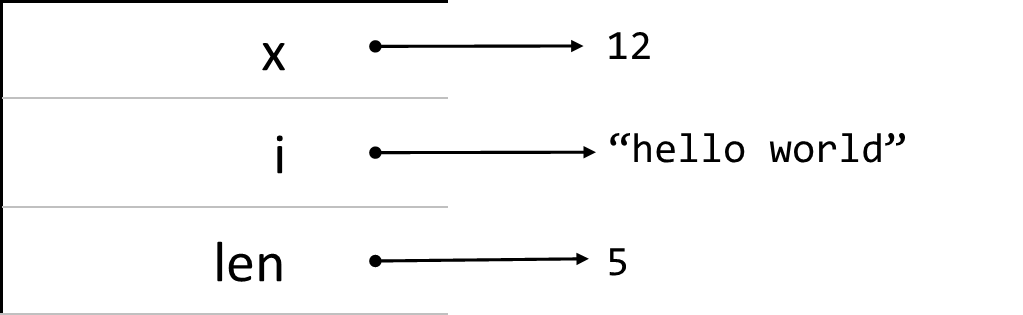
\includegraphics{diagrams/bindings-3}
  \posttabularspace

  \begin{enumerate}
    \item
\begin{verbatim}
def absVal(x):
  BODY_STATEMENTS
\end{verbatim}
    The definition creates a new local variable \expr{absVal} and assigns it to a function value with formal parameter \expr{x} and body \mvar{BODY\_STATEMENTS}.
    \pretabularspace
    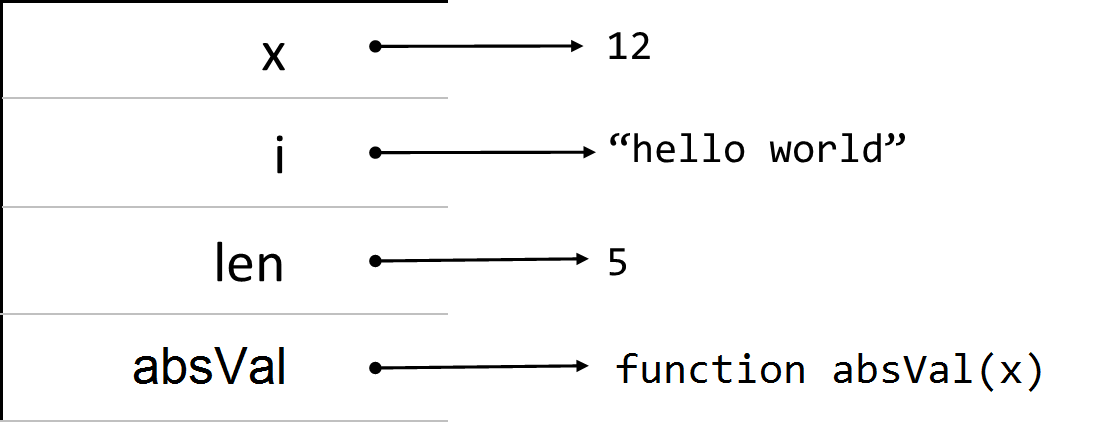
\includegraphics[scale=0.35]{diagrams/bindings-3-1}
    \posttabularspace

%     \item
% \begin{verbatim}
% def calculateGpa(class_grades, class_credits):
%   BODY_STATEMENTS
% \end{verbatim}
%     The definition creates a new local variable \expr{calculateGpa} and assigns it to a function value with formal parameters \expr{class\_grades} and \expr{class\_credits} and body \mvar{BODY\_STATEMENTS}.
%     \pretabularspace
%     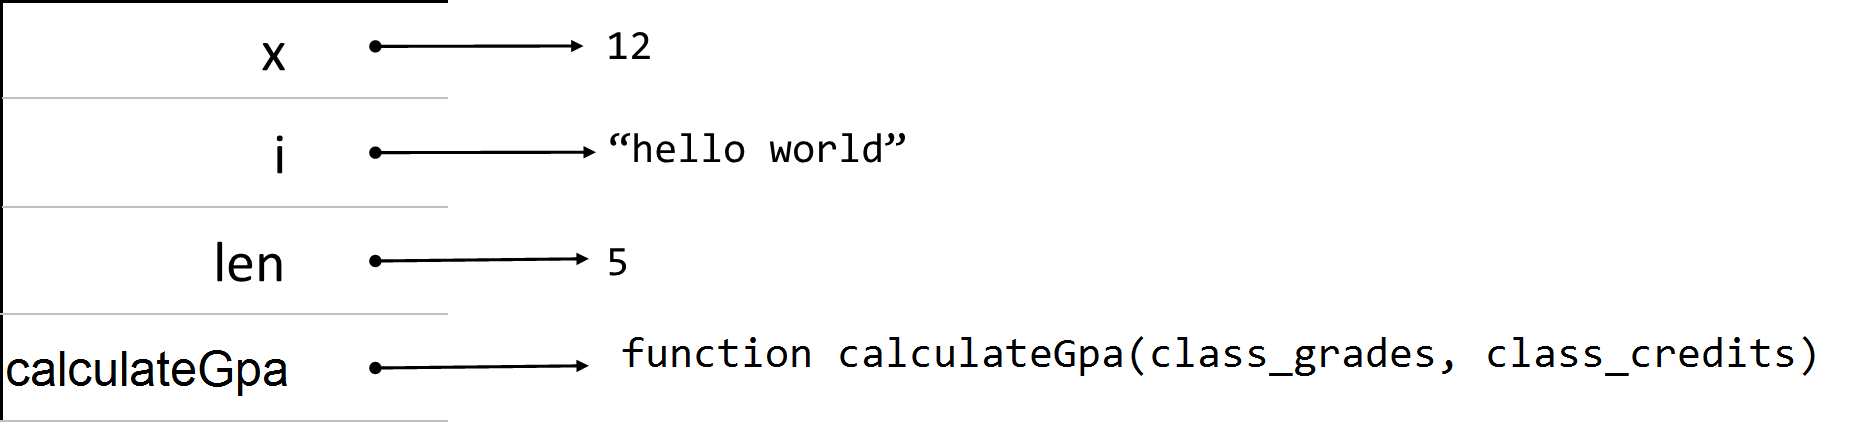
\includegraphics[scale=0.35]{diagrams/bindings-3-2}
%     \posttabularspace
%
%     \item
% \begin{verbatim}
% def str(object):
%   BODY_STATEMENTS
% \end{verbatim}
%     The definition creates a new local variable and assigns it to a function value with formal parameter \expr{object} and body \mvar{BODY\_STATEMENTS}.
%     \pretabularspace
%     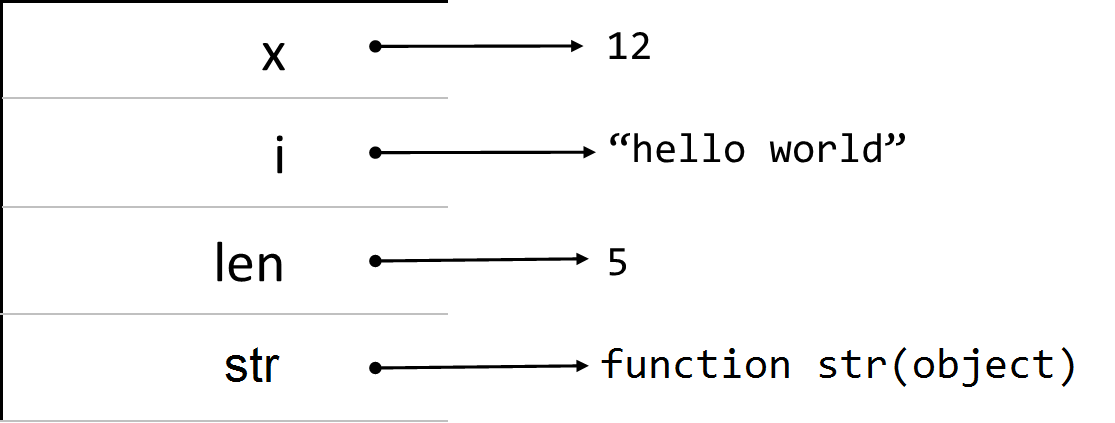
\includegraphics[scale=0.35]{diagrams/bindings-3-3}
%     \posttabularspace

    \item
\begin{verbatim}
def len(object):
  BODY_STATEMENTS
\end{verbatim}
    The definition reassigns the local variable \expr{len} and assigns it to a function value with formal parameter \expr{object} and body \mvar{BODY\_STATEMENTS}.
    \pretabularspace
    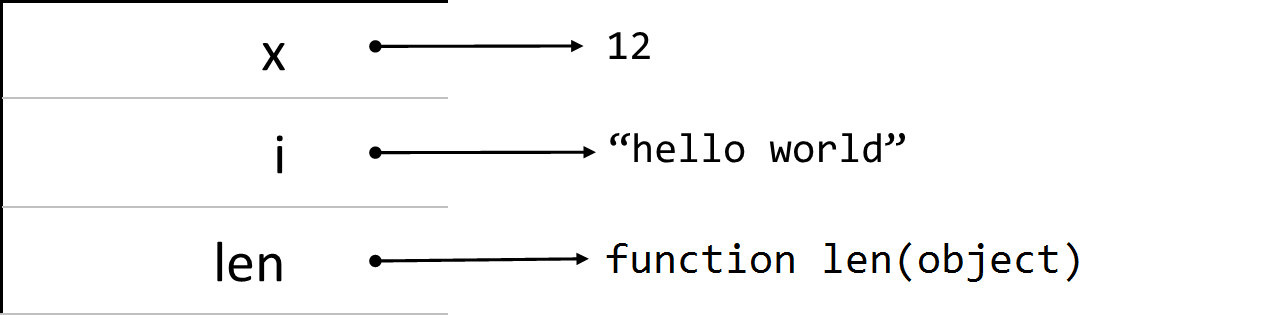
\includegraphics[scale=0.35]{diagrams/bindings-3-4}
    \posttabularspace
  \end{enumerate}


\subsection{Variable Access Expressions, Refined}
\label{accesseswithfunctions}

This section replaces Section~\ref{variableaccessexpressions} with a more
powerful set of rules.

  Recall that in general, a variable access expression such as \expr{x} has the form:

  \pretabularspace
  \mvar{VAR\_EXPR}
  \posttabularspace

  Also, recall that Python uses a structure called a frame to keep track of the variables that currently exist. In fact, Python can access and assign variables in multiple frames. These frames are arranged in a structure called an \emph{environment}, which is a list of frames.

% TODO: Add pictures!

  Each frame consists of
  \begin{itemize}
    \item A set of bindings, each of which consists of a symbol (variable) bound to a value, and
    \item A reference to its ``parent'' frame.
  \end{itemize}
  In this course, the environment always has exactly two or three frames: either
  \begin{itemize}
    \item \textbf{global} \ra built-in (built-in is global's parent), or
    \item \textbf{local} \ra global \ra built-in (global is local's parent, built-in is global's parent).
  \end{itemize} In either case, there is a ``current'' frame, where most of
  the work with variables is done. This is always the first element of the list --- either the local or the global. The current frame is bolded in the list above.

\myparagraph{The local frame is a result of function calls}
When Python executes a function call, it sets the current frame to a new,
empty local frame.  The local frame's parent is determined by where the
function's definition is.  Every function definition in this course is at
the module level, so you can assume that every local frame's parent is the
global.  (You can define a function inside a function, which would make the
local frame's parent another local frame.  This is powerful, but
potentially confusing and is beyond the scope of this course.)

  Note that a function's environment is distinct from where the function is called. This means that calling function \expr{b} from function \expr{a} does not give \expr{b} access to \expr{a}'s variables. In general, this is a good thing --- it means that functions you call can't inadvertently modify your variables.

  This new view of the Python environment complicates variable accesses and assignments. From now on, when interacting with variables, use the rules in the following sections for accesses and assignments.

\subsubsection{Rules for Evaluation}

This section replaces Section~\ref{variableaccessexpressions-rules} with a
more powerful set of rules.

  To evaluate a variable access expression,

  \begin{enumerate}
    \item
    Search the current frame for a binding for the variable
    \mvar{VAR\_EXPR}.  If you find the variable, replace the variable
    access with that variable's value.  Otherwise try the current frame's
    parent.  Continue until you either find the variable or reach the end
    of the environment.

    \item
    If you reached the end of the environment without finding the variable, raise an error --- the variable is not defined.
  \end{enumerate}

\subsubsection{Examples}

  Below are examples of evaluating variable access expressions. Each example's first line is the variable access expression, and the second is the value to which that expression evaluates.

Each example is executed in the context of this frame, unaffected by previous examples:

  \pretabularspace
  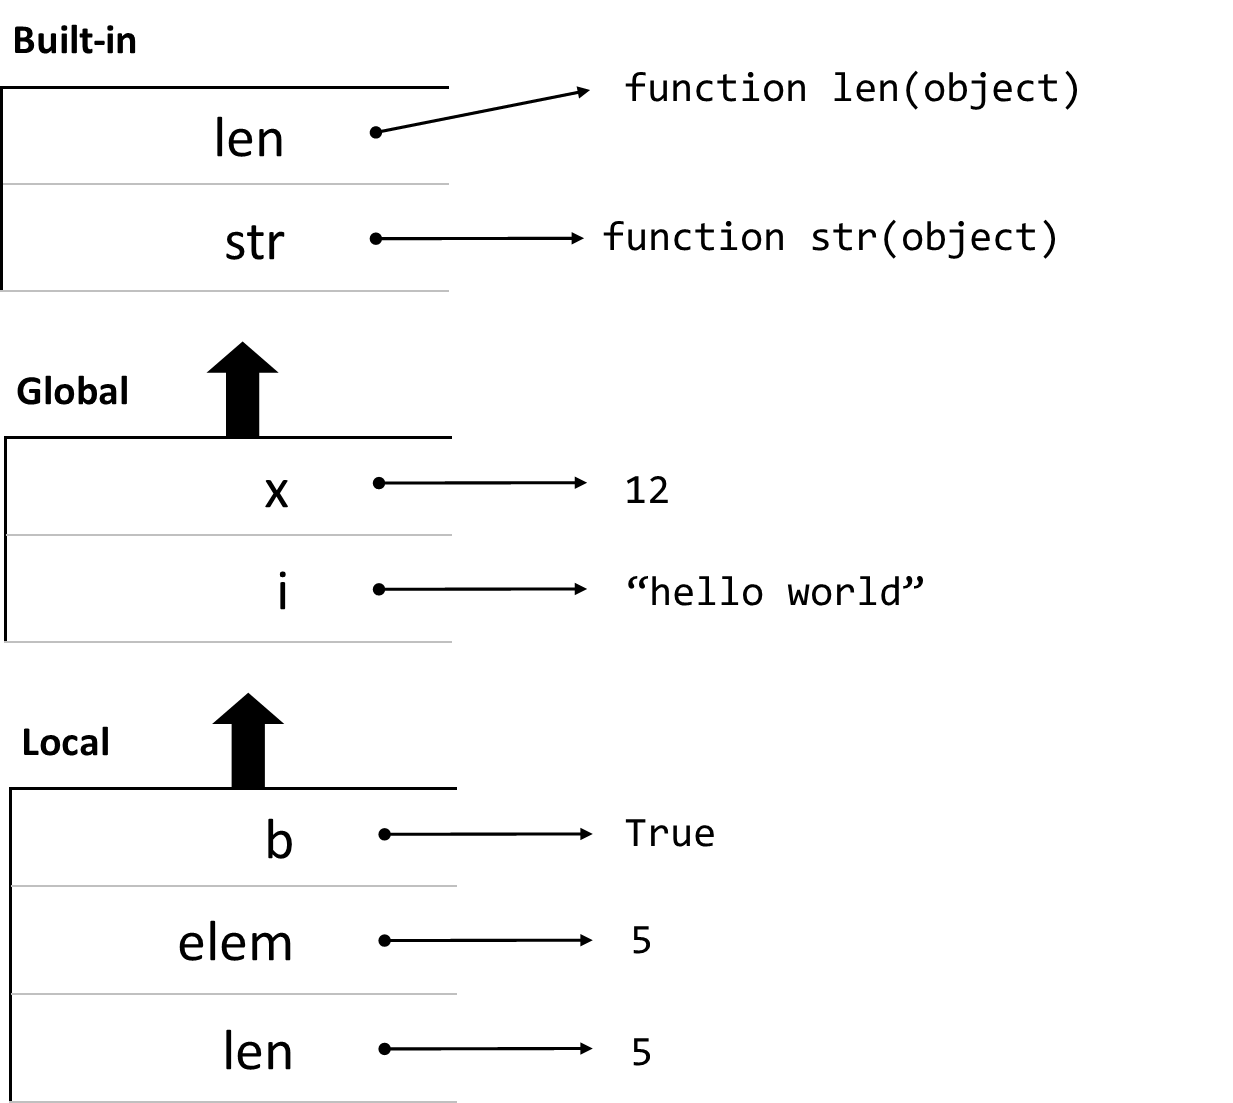
\includegraphics{diagrams/environment-1}
  \posttabularspace

  \begin{enumerate}
    \item \expr{elem} \\
    \val{5}

    \item \expr{i} \\
    \strval{hello world} \\
    After not finding \expr{i} defined in the current frame, Python
    searched the subsequent frames in the environment until finding a
    binding for \expr{i}.

    \item \expr{o} \\
    ERROR. The variable \expr{o} is not defined. \\
    Python searched each frame in the environment, but none of them had a
    binding for \expr{o}.

    \item \expr{len} \\
    \val{5}
  \end{enumerate}

\subsection{Variable Assignment Statements}
\label{assignmentswithfunctions}

This section describes the rarely-used \kw{global} keyword, which enables
you to reassign a variable in a different frame than the current one.

  Recall that in general, a variable assignment statement such as \expr{x = 18} has the form:

  \pretabularspace
  \expr{\mvar{VAR\_EXPR} = \mvar{EXPR}}

  \myparagraph{The \kw{global} keyword}
  Even in an environment with multiple frames, all variable assignments
  happen in the current frame.  Even if a variable with this name exists in
  a parent frame, a variable assignment always creates a new variable in
  the current frame and doesn't reassign the older variable.

This causes a problem when you want to reassign a variable in the global
frame from inside a function.  Instead of reassigning the global variable,
the assignment creates a new variable of the same name in the local frame.

  To assign this older variable instead of creating a new variable, precede any assignments (or accesses) to the variable with the \kw{global} statement. The global statement follows the form:

  \pretabularspace
  \expr{global \mvar{VAR\_EXPR}}
  \posttabularspace

  Where \mvar{VAR\_EXPR} is a variable in the global frame. After this statement, assigning \mvar{VAR\_EXPR} reassigns it in the global frame, not the local one.

The \kw{global} keyword does not affect variable access rules --- only
rules for reassignment.


\subsubsection{Rules for Evaluation}

  To execute a variable assignment statement,

  \begin{enumerate}

    \item
    Evaluate \mvar{EXPR} to a value and replace the expression with that value.

    \item
    Do one of the following:
    \begin{description}
      \item[If the assignment to \mvar{var\_expr} is preceded by \expr{global \mvar{var\_expr}}] Create a new variable in the global frame called \mvar{VAR\_EXPR} and give it the value from the previous step. If a variable with that name already exists in the global frame, overwrite its value with this new one.
      \item[Otherwise] Create a new variable in the local frame called \mvar{VAR\_EXPR} and give it the value from the previous step. If a variable with that name already exists in the local frame, overwrite its value with this new one.
    \end{description}
  \end{enumerate}

\subsubsection{Examples}

Below are examples of executing variable assignment statements. Each example contains one or two Python statements and a description of how those statements affect the environment.

Each example is executed in the context of this frame, unaffected by previous examples:

  \pretabularspace
  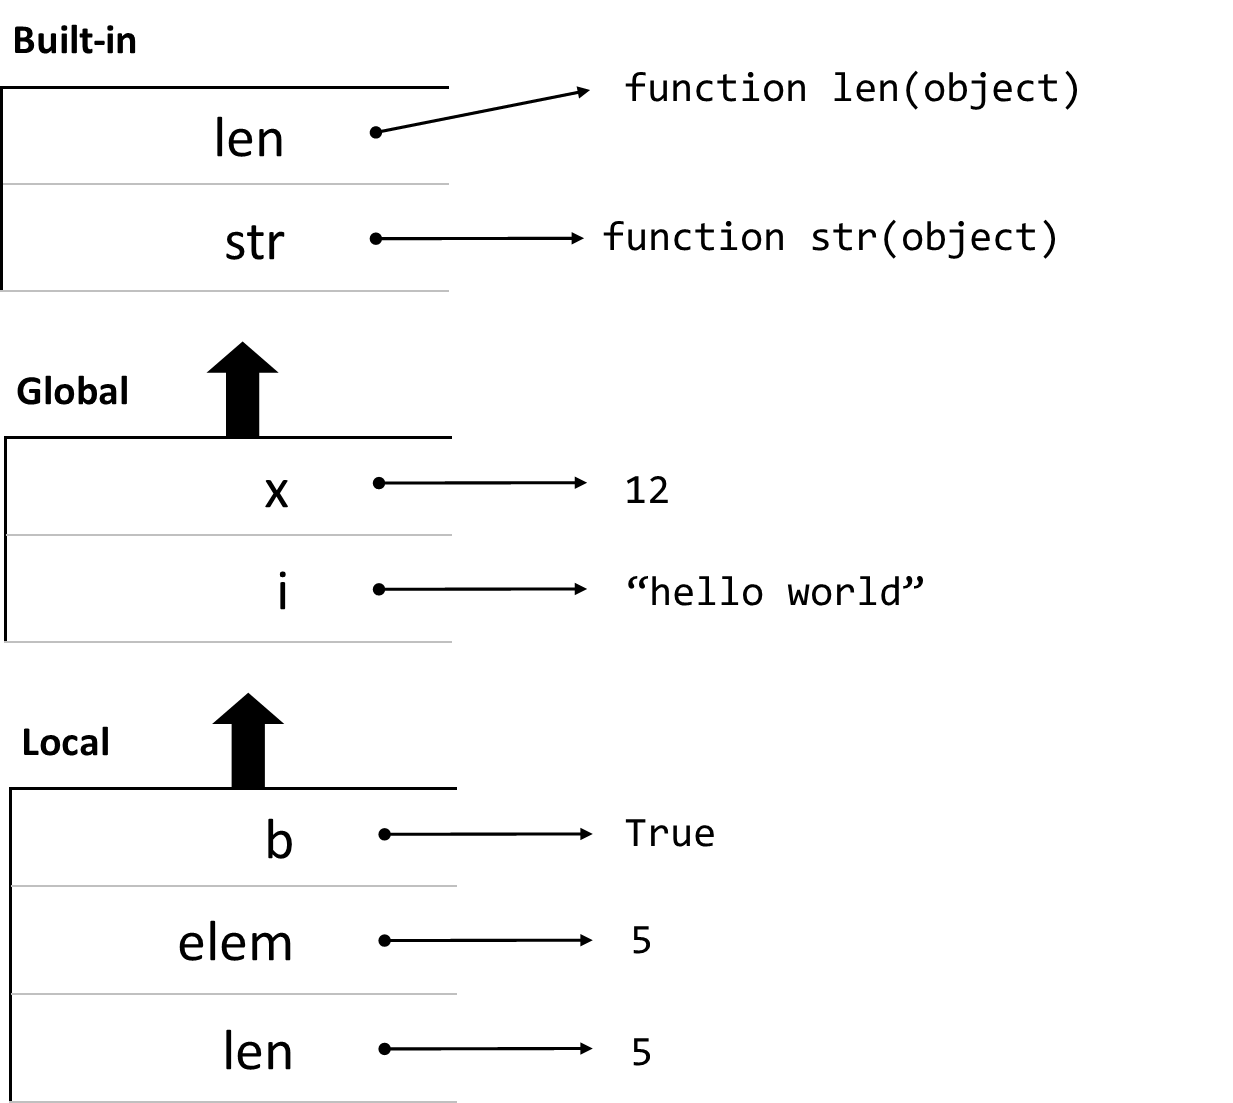
\includegraphics{diagrams/environment-1}
  \posttabularspace

% TODO: This is too many examples.  Show environment before and after?

  \begin{enumerate}
    \item \expr{var = 18} \\
    Creates \expr{var} in local frame, sets value to \val{18}.
    \item \expr{elem = x} \\
    Updates \expr{elem} in local frame, sets value to \val{12}.
    \item \expr{x = 18} \\
    Creates \expr{x} in local frame, sets value to \val{18}.
    \item \expr{len = str} \\
    Updates \expr{len} in the local frame, sets value to the value that \expr{str} has.
    \item \expr{elem = elem + 1} \\
    Updates \expr{elem} in the local frame, sets value to \val{6}.
    \item \expr{b = not b} \\
    Updates \expr{b} in the local frame, sets value to \val{False}.
    \item \expr{x = 17 + len} \\
    Creates \expr{x} in the local frame, sets value to \val{22}.
    \item \expr{elem = elem + str} \\
    ERROR. The plus operator can't operate on a function and an integer.
    \item \expr{b = b or False} \\
    Updates \expr{b} in the local frame, sets value to \val{True}.
    \item \expr{global i \\ i = \stringexpr{a string}} \\
    Updates \expr{i} in the global frame, sets value to \strval{a string}.
  \end{enumerate}

\subsection{Function Call Expressions}

  A function call expression invokes a function. Here are some examples of function calls:

  \pretabularspace
  \begin{tabular}{l c l}
  \expr{str(17) } & \Ra & \strval{17} \\
  \expr{len([1, 2, 3])} & \Ra & \val{3} \\
  \expr{abs(-1)} & \Ra & \val{1} \\
  \end{tabular}
  \posttabularspace

  In general, a function call has the form:

  \pretabularspace
  \noindent \expr{\mvar{func\_expr}(\mvar{param\_expr}, \mvar{param\_expr}, ..., \mvar{param\_expr})}
  \posttabularspace

\subsubsection{Rules for Evaluation}

% TODO: justify this:  don't trample over variables in the current frame.

When you call a function, its body is evaluated in a new, empty frame.
When the function returns, the new frame is discarded and the frame that
was the current frame for the call site is once again made the current
frame.

% When a function
% is invoked, its environment is pushed onto the stack, and becomes the current
% environment. When a function returns, its environment is popped off the stack,
% and the previous environment becomes the current one.

  To evaluate a function call,

\begin{enumerate}
\item
  At the call site (where you call the function):

  \begin{enumerate}
  \item
    Evaluate the function
    expression and replace it by the value.
  \item
    From left to right, evaluate each argument expression to a value and
    replace the expression with that value.
  \item
    If the value of the function expression is not a function value, raise
    an error.  If the number of arguments (or the names, for keyword
    arguments) is not compatible with the function's declaration, raise an
    error.  This usually requires that the number of actual arguments is
    the same as the number of formal parameters.
  \end{enumerate}

\item
  Create a new local frame for the called function.
  Make its parent the frame where the function is \emph{defined} (not where it is called).
  Make the new frame be the current frame.

\item
  In the new local frame:

  \begin{enumerate}
  \item
    Assign the actual argument values (the ones you evaluated at the call
    site) to the formal parameter variables (in the called function).  Note
    that a formal parameter variable is always a new variable in the new
    frame, not a reuse of any existing variable of the same name.

  \item
    Evaluate the body of the called function.  If you execute a \kw{return}
    statement (of the form \expr{return EXPR}), evaluate the expression to
    a value and remember the value (this is called the ``return value'').
    If the \kw{return} statement does not include an expression, then the
    return value is \kw{None}.  If you finish executing the body without
    executing a \kw{return} statement, then the return value is \kw{None}.
  \end{enumerate}

\item
  Discard the current frame, and make the previous current frame (at the
  call site) current again.

\item
  At the call site (where you call the function):
  The function call expression evaluates to the
  function's return value.  Replace the function call expression by that value.

\end{enumerate}


% TODO: Here and earlier, link to the Python Tutor!

\subsubsection{Examples}

  Below are examples of evaluating function call expressions. Each example contains a function call, the value of the function's formal parameters before executing the call, and the function's return value (the value to which the function call evaluates). In the following examples, the following functions are defined:

  \def\refmaxisbuggy{\ref{item:max-is-buggy}}

\begin{Verbatim}[commandchars=\\\{\}]
  def absVal(x):
    if x < 0:
      return -x
    return x

  # This definition overrides the built-in str function.
  def str(x):
    return len(x)

  # This definition of max is buggy, as shown in example \refmaxisbuggy below.
  def max(a, b):
    if a > b:
      return a
    elif a < b:
      return b

  def list_contains_value(lst, val):
    for element in lst:
      if element == val:
        return True
    return False

  def total_sum(lst, index):
    if index == len(lst):
      return 0
    else:
      return lst[index] + total_sum(lst, index + 1)

\end{Verbatim}

  \begin{enumerate}
    \item \expr{absVal(-7)} \\
    parameter values: \expr{x} is \val{-7} \\
    return value: \val{7}

    \item \expr{absVal(8)} \\
    parameter values: \expr{x} is \val{8} \\
    return value: \val{8}

    \item \expr{absVal(0)} \\
    parameter values: \expr{x} is \val{0} \\
    return value: \val{0}

    \item \expr{str([1, 2, 3])} \\
    parameter values: \expr{object} is \listonetwothree \\
    return value: \val{3}

    \item \expr{max(17, -8)} \\
    parameter values: \expr{a} is \val{17}, \expr{b} is \val{-8} \\
    return value: \val{17}

    \item \label{item:max-is-buggy} \expr{max(17, 17)} \\
    parameter values: \expr{a} is \val{17}, \expr{b} is \val{17} \\
    return value: \val{None}

    \item \expr{list\_contains\_value([1, 2, 3], 4)} \\
    parameter values: \expr{lst} is \listonetwothree, \expr{val} is \val{4} \\
    return value: \val{False}

    \item \expr{list\_contains\_value([], 0)} \\
    parameter values: \expr{lst} is \listzero, \expr{val} is \val{0} \\
    return value: \val{False}

    \item \expr{list\_contains\_value([\stringexpr{a}, \stringexpr{b}], \stringexpr{a})} \\
    parameter values: \expr{lst} is \listtwo{\strval{a}}{\strval{b}}, \expr{val} is \strval{a} \\
    return value: \val{True}

    \item \expr{total\_sum([], 0)} \\
    parameter values: \expr{lst} is \listzero, \expr{index} is \val{0} \\
    return value: \val{0}

    \item \expr{total\_sum([1], 0)} \\
    parameter values: \expr{lst} is \listone{1}, \expr{index} is \val{0} \\
    return value: \val{1}

    \item \expr{total\_sum([1, 2, 3], 0)} \\
    parameter values: \expr{lst} is \listonetwothree, \expr{index} is \val{0} \\
    return value: \val{6}

    \item \expr{total\_sum([], 1)} \\
    parameter values: \expr{lst} is \listzero, \expr{index} is \val{1} \\
    ERROR: list index out of range

  \end{enumerate}

\end{document}

%%% Local Variables:
%%% mode: latex
%%% TeX-master: t
%%% TeX-command-default: "PDF"
%%% End:

%  LocalWords:  EXPR mylist expr elif BOOL timeline unordered lst mydict
%  LocalWords:  mytuple len DS eft ight del lst4 KeyError og ay struct str
%  LocalWords:  param1 param2 param absVal global's bolded func
